\documentclass{ieeetj}
\usepackage{cite}
\usepackage{amsmath,amssymb,amsfonts}
\usepackage{algorithmic}
\usepackage{graphicx,color}
\usepackage{textcomp}
\usepackage{xcolor}
\usepackage{hyperref}
\usepackage{xcolor}
\usepackage{longtable}
\usepackage{booktabs}
\usepackage{array}
\usepackage{caption}
\usepackage{ragged2e}
\usepackage{svg}
\makeatletter
\let\labelindent\relax
\makeatother
\usepackage{enumitem}
\hypersetup{hidelinks}
\usepackage{algorithm,algorithmic}
\usepackage{multirow}
\def\BibTeX{{\rm B\kern-.05em{\sc i\kern-.025em b}\kern-.08em
    T\kern-.1667em\lower.7ex\hbox{E}\kern-.125emX}}
\AtBeginDocument{\definecolor{tmlcncolor}{cmyk}{0.93,0.59,0.15,0.02}\definecolor{NavyBlue}{RGB}{0,86,125}}

\newcommand{\mfabric}{M\textsuperscript{2}Fabric}

\def\OJlogo{\vspace{-4pt}$<$Society logo(s) and publication title will appear here.$>$}
\def\seclogo{\vspace{10pt}$<$Society logo(s) and publication title will appear here.$>$}

\def\authorrefmark#1{\ensuremath{^{\textbf{#1}}}}

\begin{document}
\receiveddate{XX Month, XXXX}
\reviseddate{XX Month, XXXX}
\accepteddate{XX Month, XXXX}
\publisheddate{XX Month, XXXX}
\currentdate{XX Month, XXXX}
\doiinfo{XXXX.2022.1234567}

\markboth{M\textsuperscript{2}FABRIC: A MULTILAYER POST-QUANTUM CRYPTOGRAPHIC ARCHITECTURE FOR HYPERLEDGER FABRIC}{CHEONG {ET AL.}} 

\title{\mfabric{}: A Multilayer Post-Quantum Cryptographic Architecture for Hyperledger Fabric}

\author{Zara Laila Cheong\authorrefmark{1}, Ali Tufail\authorrefmark{1}, and Rosyzie Anna Apong\authorrefmark{1}}
\affil{School of Digital Science, Universiti Brunei Darussalam, Bandar Seri Begawan, BE1410, Brunei Darussalam}
\corresp{Corresponding author: Zara Laila Cheong (email: zaralaila@icloud.com).}
\authornote{The authors declare no specific funding for this work and no conflicts of interest. The implementation, benchmark scripts, and measurement data are openly available in the M\textsuperscript{2}Fabric repository to support independent reproduction.}


\begin{abstract}
{Hyperledger Fabric relies on classical elliptic-curve cryptography across its
entire transaction lifecycle and identity infrastructure, making every signing,
certification, validation, and key-exchange operation vulnerable to a
cryptographically relevant quantum computer. Prior post-quantum proposals for
Fabric have each addressed only a subset of its cryptographic layers, leaving
the unaddressed layers quantum-exploitable. This article presents \mfabric{}, a
multilayer post-quantum architecture that replaces all four live cryptographic
layers of Hyperledger Fabric v2.5.12 and Fabric CA v1.5.12 simultaneously: the
Blockchain Cryptographic Service Provider (BCCSP) signing layer, the
certificate infrastructure, the Membership Service Provider
identity-validation layer, and the Transport Layer Security (TLS) inter-node
transport layer. The design uses the NIST-standardised algorithms ML-DSA-44
(FIPS~204, Category~2), ML-DSA-65 (FIPS~204, Category~3), FN-DSA-512
(FIPS~206 Initial Public Draft, Category~1), and ML-KEM-768 (FIPS~203,
Category~3) through pure-Go libraries and is deployed in three migration
phases. The principal engineering contribution is \textit{buildPQCChain()},
a certificate-chain validator that bypasses the Go standard library's
rejection of post-quantum object identifiers, enabling a live certificate
authority to issue and validate post-quantum certificates at runtime. The
implementation is verified through NIST Automated Cryptographic Validation
Protocol (ACVP) coverage, interface-compliance
tests, round-trip tests, and end-to-end transaction execution with zero
failures. An empirical evaluation on a two-organisation network using
Hyperledger Caliper v0.6.0 ($n=27$ benchmark runs per workload across nine
algorithm-phase combinations plus a six-run ECDSA baseline) shows that the
complete Phase~3 deployment reduces maximum sustainable write-heavy
throughput from a 275.3~TPS ECDSA baseline by only 3.5 percent for
FN-DSA-512, 10.9 percent for ML-DSA-44, and 18.0 percent for ML-DSA-65,
with bootstrap and Cohen's-$d$ checks supporting the headline ordering. The
results establish per-endorsement payload size, not signing speed, as the
dominant throughput determinant.}
\end{abstract}

\begin{IEEEkeywords}
{Blockchain security, certificate chain validation, crypto-agility,
Hyperledger Fabric, ML-DSA, ML-KEM, post-quantum cryptography, quantum-resistant
key exchange.}
\end{IEEEkeywords}

\maketitle

%=====================================================================
\section{Introduction} \label{sec:intro}
%=====================================================================
\IEEEPARstart{H}{yperledger} Fabric's quantum vulnerability is complete and
uniform across all twenty-five cryptographic operations identified in the
transaction lifecycle and identity-management infrastructure. The central
challenge of this work is to translate eight formal integration requirements,
derived from a threat analysis of those operations, into source-code
modifications to Hyperledger Fabric v2.5.12 and Fabric Certificate Authority v1.5.12 that replace
all four live cryptographic layers with NIST-standardised post-quantum
equivalents while preserving functional compatibility with the Fabric component
ecosystem.

The four layers requiring simultaneous replacement are the BCCSP signing layer,
which provides digital-signature services to all Fabric components; the
certificate infrastructure layer, which issues and validates X.509 identity
certificates; the MSP identity-validation layer, which authenticates
participants at runtime; and the TLS inter-node communication layer, which
protects all inter-component network traffic. Prior work has addressed subsets
of these layers in
isolation~\cite{holcomb2021, hu2025prototype, abbas2025, kasula2025, razdan2025postquantum},
but no published implementation has addressed all four simultaneously. As
established by the threat analysis underlying this work, partial integration
creates a structural vulnerability in which the unaddressed layers remain
quantum-exploitable regardless of the post-quantum strength of the addressed
layers.

The implementation presented here, \mfabric{}, provides a post-quantum BCCSP
plugin supporting ML-DSA-44, ML-DSA-65, and FN-DSA-512 through constant-time
pure-Go libraries; extends the live Fabric CA to issue X.509 certificates
carrying post-quantum public keys; implements a custom object-identifier
(OID)-aware certificate-chain validator in the MSP without modifying the
Go standard library; and
activates ML-KEM-768 hybrid key exchange at the TLS layer. All four
modifications are verified through NIST ACVP test vectors, Fabric
interface-compliance tests and end-to-end transaction lifecycle execution. This article makes the following contributions beyond
the existing post-quantum Hyperledger Fabric literature:

\begin{itemize}
\item \textbf{Multilayer post-quantum integration.} To the authors'
knowledge, the first runtime implementation to address the four primary
cryptographic layers of Fabric v2.5.x (BCCSP signing, certificate
infrastructure, MSP identity validation, and TLS transport) simultaneously
using FIPS-standardised algorithms (FIPS~203, 204, and the FIPS~206 Initial
Public Draft) in unmodified Go.

\item \textbf{The \textit{buildPQCChain()} certificate chain validator.} A
self-contained OID-dispatched validator that solves the practical barrier
created by Go's standard library X.509 implementation rejecting certificate
chains carrying post-quantum OIDs, a barrier that has prevented live
certificate-authority integration in prior
work~\cite{holcomb2021, hu2025prototype, abbas2025}.

\item \textbf{End-to-end performance characterisation on the current LTS.}
The first end-to-end performance characterisation of a four-layer
FIPS-standardised integration on Hyperledger Fabric v2.5.12 ($n=27$ benchmark
runs per workload across 9 algorithm-phase combinations, plus a 6-run ECDSA
baseline), establishing per-endorsement payload size, not signing speed, as
the dominant throughput determinant.

\item \textbf{Resolution of practical engineering barriers.} The
implementation also reveals and resolves engineering challenges not apparent
from a high-level design analysis: Go's rejection of post-quantum OIDs
requires a bypass for both certificate generation and chain validation;
FN-DSA's variable-length signatures require careful handling in Fabric's
serialisation code; and the post-quantum certificate authority extension
must integrate with the existing CFSSL signing pipeline through a
registered hook rather than a parallel code path.
\end{itemize}

The remainder of this article is organized as follows.
Section~\ref{sec:litreview} reviews prior post-quantum Fabric integrations and
the relevant cryptographic and standardisation background.
Section~\ref{sec:methodology} presents the methodology: the construction
approach, the design requirements and principles, the post-quantum algorithm
selection, the four-layer architecture and three-phase migration, and the
implementation of each layer. Section~\ref{sec:experimental} describes the
experimental setup, test network, verification procedure, and benchmark
methodology, and reports the verification and performance results, the
consolidated statistical analysis, and a security analysis of the
implementation. Section~\ref{sec:discussion} discusses completeness,
generalisability, alignment with national PQC migration strategies, and
limitations. Section~\ref{sec:conclusion} concludes, consolidating the
limitations and future-work agenda.

%=====================================================================
\section{Literature Review} \label{sec:litreview}
%=====================================================================

The background relevant to \mfabric{} spans three areas: the standardisation
of post-quantum cryptographic primitives by NIST and its international
counterparts, the practical performance and deployment of post-quantum TLS,
and prior post-quantum integrations of Hyperledger Fabric. This section
reviews each in turn. The review identifies a recurring gap that the
remaining sections of this article address: prior Fabric integrations have
each replaced a strict subset of the platform's cryptographic layers,
leaving the unaddressed layers quantum-exploitable irrespective of the
strength of the layers that were replaced.

\subsection{Post-Quantum Cryptography and Standardisation}

The threat that a cryptographically relevant quantum computer (CRQC)
poses to classical public-key cryptography motivates the migration to
post-quantum algorithms. Shor's algorithm renders the elliptic-curve discrete-logarithm
problem (ECDLP) and integer factorisation tractable, breaking ECDSA, ECDH, and
RSA. In response, NIST conducted a six-year standardisation process that
subjected candidate algorithms to international
cryptanalysis~\cite{alagic2022nist}, culminating in FIPS~203 (ML-KEM, key
encapsulation)~\cite{nist_fips203}, FIPS~204 (ML-DSA, lattice
signatures)~\cite{nist_fips204}, FIPS~205 (SLH-DSA, hash-based
signatures)~\cite{nist_fips205}, and the FIPS~206 Initial Public Draft
(FN-DSA, NTRU-lattice signatures)~\cite{nist_fips206}. ML-DSA derives from the CRYSTALS-Dilithium
construction over module lattices~\cite{ducas2018dilithium}, and FN-DSA from the
Falcon construction over NTRU lattices~\cite{pornin2019, prest2020falcon}. NIST
guidance on transitional security recommends hybrid
constructions~\cite{barker2020transition}, an approach formalised for signatures
by Bindel et al.~\cite{bindel2017} and instantiated for TLS key exchange by the
IETF hybrid framework~\cite{ietf_hybrid_tls} and the
\textit{X25519MLKEM768} codepoint~\cite{ietf_x25519mlkem768}. A persistent
practical concern is side-channel resistance: the systematic survey of Ravi et
al.~\cite{ravi2024sidechannel} catalogues power-analysis, electromagnetic, and
fault-injection attacks against lattice schemes and confirms that constant-time
arithmetic, while necessary, is not sufficient for adversarial
deployment~\cite{pessl2019}.

\subsection{Post-Quantum TLS}

The performance of post-quantum TLS has been characterised independently by
Paquin et al.~\cite{paquin2020benchmark} and Sikeridis et al.~\cite{sikeridis2020},
both of whom found that the principal cost is the increase in handshake bandwidth
from larger KEM ciphertexts and signature payloads, while per-operation
cryptographic computation contributes negligibly relative to network round-trip
time. These TLS-level findings establish that the dominant cost of post-quantum
transport security is payload-driven, a theme that recurs at the
application layer in the present work. The Open Quantum Safe project's
\textit{liboqs} library~\cite{stebila2016oqs} and Cloudflare's CIRCL library
provide the reference implementations against which integration work is built;
CIRCL's pure-Go ML-DSA and ML-KEM run in production at Cloudflare scale with
independent security review.

\subsection{Post-Quantum Hyperledger Fabric}

Hyperledger Fabric~\cite{androulaki2018} is a permissioned blockchain whose
transaction throughput under classical cryptography has been characterised by
Baliga et al.~\cite{baliga2018performance}, Kuzlu et
al.~\cite{kuzlu2021performance}, Nasir et al.~\cite{nasir2018}, and Thakkar et
al.~\cite{thakkar2018}, whose analyses identify endorsement-signature
verification at the committing peer as a principal scaling bottleneck. 

Prior post-quantum work on Hyperledger Fabric falls into four categories.
\emph{Algorithm benchmarks without Fabric integration} are exemplified by
Campbell~\cite{campbell2019, campbell2019eval}, who evaluated qTESLA
against ECDSA for healthcare and GDPR contexts but produced no running
implementation; qTESLA was subsequently dropped from
NIST~Round~3~\cite{alagic2022nist}. \emph{Attack-surface surveys} are
represented by Brotsis et al.~\cite{brotsis2020}, whose IoT-forensics
study catalogues quantum-vulnerable Fabric components without proposing
an integration. \emph{Application-layer integrations} place post-quantum
primitives in chaincode or trusted enclaves while leaving Fabric's BCCSP,
CA, MSP, and TLS classical: Lee~\cite{lee2025} provides ML-DSA, Vesper,
and TDUE as Fabric Private Chaincode services under Intel~SGX; Das et
al.~\cite{das2025genomic} embed CRYSTALS-Kyber and Dilithium in genomic
data chaincode; Revathi and Suganthi~\cite{revathi2025} embed Kyber,
Falcon, and Dilithium in hospital-data chaincode. \emph{Endorsement-policy
proxies} configure multiple-organisation signatures as a governance
control rather than a cryptographic replacement: Razdan and
Nene~\cite{razdan2025postquantum} report a 119\% latency increase under a
dual-signature endorsement policy on standard Fabric, with no
modification of cryptographic primitives.

The four \emph{infrastructure-layer integrations} (Kasula et
al.~\cite{kasula2025}, PQFabric (Holcomb et al.)~\cite{holcomb2021},
Abbas et al.~\cite{abbas2025}, and Hu~\cite{hu2025prototype}) each
address a strict subset of Fabric's four cryptographic layers.
Kasula et al.'s Fabric-LPQC~\cite{kasula2025} integrated the SM2/SM3/SM4
national algorithms with NIST Round~3 candidates into the Fabric~1.4
BCCSP; SM2, the signature scheme it presents as ``post-quantum,'' is
elliptic-curve-based and therefore equally vulnerable to Shor's
algorithm. PQFabric~\cite{holcomb2021} replaced the Fabric~1.4 signature
layer via CGo (the Go-to-C foreign-function interface) bindings to
\textit{liboqs} with pre-FIPS parameters and
established that per-payload overhead, not signing speed, dominates
performance, an observation that \mfabric{} extends to the FIPS-finalised
generation. Abbas et al.~\cite{abbas2025} added post-quantum certificate
generation to the offline Cryptogen tool but did not address the live CA,
TLS, or MSP chain validation. Hu~\cite{hu2025prototype} targeted
Fabric~3.0 but required a non-standard Go compiler fork and used offline
Cryptogen-generated certificates with pre-FIPS algorithms.

The common limitation across all four is the incompatibility between
post-quantum OIDs and Go's \textit{crypto/x509}, which has confined prior
work to offline certificate generation and left the live CA's classical
signing key active. This is the residual identity-CA vulnerability that
motivates the multilayer approach. \mfabric{} resolves this barrier directly and is,
to the authors' knowledge, the first integration to address all four live
cryptographic layers of the current Fabric LTS simultaneously using
FIPS-standardised algorithms in unmodified Go.
Table~\ref{tab:prior_work_comparison} consolidates the coverage of each
prior work against the four-layer decomposition. In the table, the
checkmark indicates that the layer is fully addressed at runtime;
``offline'' indicates that the layer is addressed only via offline
certificate generation, with the live CA's classical signing key still
active; ``app.'' indicates that post-quantum primitives are applied at the
application layer (in chaincode or in a trusted enclave) above the Fabric
infrastructure; ``proxy'' indicates an endorsement-policy mechanism rather
than a cryptographic replacement; and the dash indicates that the layer is
not addressed or not applicable to the prior work in question. The
Standard Go column indicates whether the implementation builds under
unmodified Go without compiler forks or CGo bindings.

Two entries warrant explicit qualification. Campbell evaluated qTESLA,
which was eliminated from NIST PQC Round~3
standardisation~\cite{alagic2022nist}; the evaluation also provided
algorithm benchmarks only, without Fabric integration. Kasula et al.'s
primary signature algorithm SM2 is elliptic-curve-based and is therefore
equally vulnerable to Shor's algorithm, so the framing of SM2 as
``post-quantum'' is technically incorrect; the work also lists
CRYSTALS-Dilithium, CRYSTALS-Kyber, FALCON, and SPHINCS+ as alternatives
without integrating them at the BCCSP level. Regarding algorithm choice,
PQFabric and Hu used pre-FIPS lattice parameters, whereas \mfabric{} uses
ML-DSA-44, ML-DSA-65 (both FIPS~204), FN-DSA-512 (FIPS~206 Initial Public
Draft), and ML-KEM-768 (FIPS~203). For the transport layer, \mfabric{}
activates the standardised \textit{X25519MLKEM768} hybrid key exchange
via Go~1.24's \textit{crypto/tls}. Empirically, \mfabric{} reports
$n=27$ benchmark runs per workload (nine algorithm-phase combinations
across three repetitions) together with a six-run ECDSA baseline.

\begin{table*}[ht]
\centering
\caption{Coverage comparison of prior post-quantum Hyperledger Fabric
work.}
\label{tab:prior_work_comparison}
\setlength{\tabcolsep}{4pt}
\footnotesize
\begin{tabular}{@{}>{\raggedright\arraybackslash}p{5.5cm} c c c c c c c c c@{}}
\toprule
\textbf{Work} & \textbf{Fabric}
& \textbf{BCCSP} & \textbf{Certificate} & \textbf{Live} & \textbf{MSP}
& \textbf{TLS} & \textbf{FIPS} & \textbf{Standard}
& \textbf{Empirical} \\
& \textbf{Version}
& \textbf{Signing} & \textbf{Infrastructure} & \textbf{CA} & \textbf{Validation}
& \textbf{Layer} & \textbf{Algorithm} & \textbf{Go}
& \textbf{Evaluation} \\
\midrule
\multicolumn{10}{@{}l@{}}{\textit{\textbf{Algorithm benchmarking without Fabric integration}}} \\
Campbell~\cite{campbell2019, campbell2019eval}                          & --    & --        & --      & --        & --        & --        & qTESLA                    & --        & benchmark \\
\addlinespace
\multicolumn{10}{@{}l@{}}{\textit{\textbf{Fabric attack-surface survey, no implementation}}} \\
Brotsis et al.~\cite{brotsis2020}                                       & --    & --        & --      & --        & --        & --        & survey                    & --        & --        \\
\addlinespace
\multicolumn{10}{@{}l@{}}{\textit{\textbf{Application-layer / chaincode / enclave (Fabric infrastructure unchanged)}}} \\
Lee (SGX)~\cite{lee2025}                                                & 2.x    & app.      & --      & --        & --        & --        & \checkmark                & partial   & partial   \\
Das et al.~\cite{das2025genomic}                                        & 2.x    & app.      & --      & --        & --        & --        & \checkmark                & --        & partial   \\
Revathi \& Suganthi~\cite{revathi2025}                                  & 2.x    & app.      & --      & --        & --        & --        & partial                   & --        & partial   \\
\addlinespace
\multicolumn{10}{@{}l@{}}{\textit{\textbf{Endorsement-policy governance proxy (not a cryptographic replacement)}}} \\
Razdan \& Nene~\cite{razdan2025postquantum}                             & 2.x    & proxy     & --      & --        & --        & --        & partial                   & --        & partial   \\
\addlinespace
\multicolumn{10}{@{}l@{}}{\textit{\textbf{Fabric infrastructure-layer integrations}}} \\
Fabric-LPQC (Kasula et al.)~\cite{kasula2025}                           & 1.4    & \checkmark & --      & --        & --        & --        & --                        & partial   & partial   \\
PQFabric (Holcomb et al.)~\cite{holcomb2021}                            & 1.4    & \checkmark & offline & --        & --        & --        & --                        & --        & \checkmark \\
Abbas et al.~\cite{abbas2025}                                           & 2.x    & \checkmark & offline & --        & --        & --        & \checkmark                & \checkmark & --        \\
Hu (prototype)~\cite{hu2025prototype}                                   & 3.0    & \checkmark & offline & --        & --        & --        & --                        & --        & partial   \\
\addlinespace
\midrule
\textbf{\mfabric{}}
                                                                        & \textbf{2.5.12}     & \textbf{\checkmark} & \textbf{\checkmark} & \textbf{\checkmark}
                                                                        & \textbf{\checkmark} & \textbf{\checkmark} & \textbf{\checkmark} & \textbf{\checkmark}
                                                                        & \textbf{\checkmark} \\
\bottomrule
\end{tabular}
\end{table*}

%=====================================================================
\section{Methodology} \label{sec:methodology}
%=====================================================================

This section presents the construction methodology, the formal design
requirements and principles, the post-quantum algorithm selection, the
four-layer architecture and three-phase migration design, and the implementation
of each cryptographic layer.

\subsection{Construction Methodology}
\label{sec:method_construction}

The implementation follows the design-science
artefact-construction methodology, translating the eight integration
requirements derived from the threat analysis into a working system through
a requirements-to-design-principles-to-implementation chain in which every
significant decision is traceable to a design principle and thence to a
requirement (\textit{Design Requirements and Principles} subsection of
the \textit{Methodology} section).

The target platform is Hyperledger Fabric v2.5.12 (commit \textit{af0b647})
and Fabric CA v1.5.12, selected as the recommended production LTS branch.
Cloudflare CIRCL v1.6.3 provides pure-Go ML-DSA-44, ML-DSA-65, and
ML-KEM-768~\cite{nist_fips203, nist_fips204}; \textit{go-fn-dsa} v0.2.0
provides FN-DSA-512 from the FIPS~206 Initial Public
Draft~\cite{nist_fips206}. Go~1.24 is the minimum required version (it
introduced \textit{tls.X25519MLKEM768}, replacing the pre-standard
\textit{X25519Kyber768Draft00} from Go~1.23); benchmark binaries are
pinned to Go~1.24 for reproducibility. The implementation is structured
as non-invasive patches preserving existing module structure, interface
contracts, and test coverage, introducing post-quantum functionality
through new files and types rather than modification of existing functions
wherever feasible.

\subsection{Design Requirements and Principles}
\label{sec:method_principles}

The eight formal integration requirements~R1--R8 derived from the
threat-analysis foundation of this work are reproduced in
Table~\ref{tab:requirements_principles}, paired one-to-one with the eight
design principles~DP1--DP8 that govern every significant implementation
decision. The requirements address five threat scenarios identified by
the threat analysis: TS1 (identity impersonation via certificate
forgery), TS2 (transaction-signature forgery), TS3 (block-integrity
compromise via orderer key recovery), TS4 (TLS session decryption via
harvest-now-decrypt-later (HNDL)), and TS5 (gossip-protocol manipulation). Each
design choice in the remainder of this section is traceable to a DP and
thence to an R, and ultimately to one or more threat scenarios. The
requirements derive from the threat analysis that motivates this work;
the design principles translate them into engineering decisions guiding
the implementation. Cross-references in the \textit{BCCSP Layer
Implementation}, \textit{Certificate Infrastructure Implementation},
\textit{MSP Identity Validation}, and \textit{TLS Layer Implementation}
subsections of the \textit{Methodology} section cite the DP or R that
each decision satisfies.

\begin{table*}[ht]
\centering
\caption{Formal integration requirements and design principles.}
\label{tab:requirements_principles}
\setlength{\tabcolsep}{5pt}
\footnotesize
\begin{tabular}{@{}c>{\raggedright\arraybackslash}p{5.5cm}>{\raggedright\arraybackslash}p{11.5cm}@{}}
\toprule
\textbf{\#} & \textbf{Threat Analysis Requirement} & \textbf{Design Principle (engineering translation)} \\
\midrule
1 & PQC signing at all lifecycle signing points (TS2, TS3)
  & Replace the BCCSP signing backend rather than its call sites;
    all peer/orderer/client signing paths reach PQC by configuration alone. \\
2 & PQC key encapsulation for TLS sessions (TS4 / TLS component of TS5)
  & Use the standardised hybrid \textit{X25519MLKEM768}
    named-curve constant exposed by the Go~1.24 \textit{crypto/tls}
    package; no in-process key-exchange code. \\
3 & Runtime PQC certificate issuance by the Fabric CA (TS1)
  & Bypass Go's \textit{x509.CreateCertificate} and
    \textit{x509.Certificate.Verify} via custom ASN.1 DER
    construction and the OID-dispatched
    \textit{buildPQCChain()} validator. \\
4 & Preserve the BCCSP interface contract
  & Implement PQC behaviour through a new factory/backend pair;
    do not modify the \textit{bccsp.BCCSP} interface or any caller. \\
5 & Cryptographic agility via configuration
  & Make algorithm dispatch table-driven (registry map keyed by
    OID and algorithm name); new algorithms require only a new
    entry, not new code paths. \\
6 & Functional correctness across the transaction lifecycle
  & Validate via NIST ACVP coverage, round-trip integration
    tests, interface-compliance tests, and end-to-end
    transaction execution in all three migration phases. \\
7 & Constant-time implementation discipline
  & Inherit constant-time guarantees from Cloudflare CIRCL and
    \textit{go-fn-dsa}; characterise residual side-channel
    surface for HSM deployment in follow-up work. \\
8 & Phased migration without simultaneous-upgrade requirement
  & Stage the integration across three phases (BCCSP-only $\to$
    +certificate infrastructure $\to$ +hybrid TLS) so that the
    residual quantum-attack surface decreases monotonically per
    Eq.~(\ref{eq:residual_surface}). \\
\bottomrule
\end{tabular}
\end{table*}

DP3 is the most technically demanding principle because it requires bypassing
Go's standard-library X.509 certificate-generation API for post-quantum keys;
the \textit{buildPQCChain()} validator of the \textit{MSP Identity
Validation} subsection of the \textit{Methodology} section is a direct
consequence, since a live CA that issues post-quantum certificates
requires a live validator that can verify them. For DP7, the survey of Ravi
et al.~\cite{ravi2024sidechannel} confirms that constant-time arithmetic is
necessary but not sufficient for adversarial deployment; the residual
power-analysis, electromagnetic, and fault-injection surface is outside the
scope of an infrastructure-level integration but is the subject of the
adversarial workstream described in the \textit{Planned
Adversarial-Evaluation Workstream} subsection of the \textit{Experimental
Setup and Results} section.

The multilayer coverage objective can be stated formally. Let
$\mathcal{L}=\{\ell_1,\dots,\ell_4\}$ be the set of quantum-vulnerable
cryptographic layers and let $x_{\ell}\in\{0,1\}$ indicate whether layer $\ell$
is migrated to a post-quantum primitive. DP1--DP8 jointly require the coverage
constraint

\begin{equation}
\sum_{\ell\in\mathcal{L}} x_{\ell} = |\mathcal{L}| = 4 ,
\label{eq:coverage_constraint}
\end{equation}

where $x_{\ell}$ is the binary migration indicator for layer $\ell$ and
$|\mathcal{L}|$ is the number of vulnerable layers. Any solution with
$\sum_{\ell} x_{\ell}<4$ leaves at least one layer quantum-exploitable; the
multilayer design exists precisely to satisfy~(\ref{eq:coverage_constraint})
with equality, distinguishing \mfabric{} from the partial integrations of prior
work.

\subsection{Post-Quantum Algorithm Selection}
\label{sec:method_alg}

Having fixed the design principles, the next step is to select the concrete
algorithms that instantiate them. The selection is constrained by R1 to
NIST-standardised algorithms from FIPS~203, 204, 205, or 206, and is then guided
by four criteria: security-level appropriateness, anticipated blockchain
performance, availability of production-quality pure-Go implementations, and
compatibility with Go's certificate and TLS infrastructure.

\subsubsection{Selection Cost Model}

To make the selection criterion explicit, define for a candidate signature
algorithm $a$ a deployment cost

\begin{equation}
C(a) \;=\; w_{p}\,\Pi(a) \;+\; w_{s}\,\frac{1}{\kappa(a)} \;-\; w_{c}\,\mathbb{1}_{\mathrm{Go}}(a),
\label{eq:selection_cost}
\end{equation}

where $\Pi(a)=|\sigma_a|+|\mathit{cert}_a|$ is the per-endorsement payload
(the sum of the signature length $|\sigma_a|$ and the endorser's DER-encoded
X.509 certificate length $|\mathit{cert}_a|$, which includes the holder's
public key, the issuer's signature on the TBS structure, and the RFC~5280
envelope), $\kappa(a)\in\{1,2,3,5\}$ is the NIST security category,
$\mathbb{1}_{\mathrm{Go}}(a)$ is unity when a production pure-Go implementation
exists and zero otherwise, and $w_p,w_s,w_c\ge 0$ are weights encoding the
deployment's relative emphasis on payload, security margin, and tooling
simplicity. The minus sign on the third term encodes a \emph{bonus}, not a
cost: a candidate with a production pure-Go implementation lowers $C(a)$
because it removes the CGo-toolchain dependency, cross-language memory
management, and the constant-time-on-the-FFI-boundary concern that would
otherwise inflate integration risk. The blockchain context drives $w_p$
high because $\Pi(a)$ is paid on every endorsement in every block, whereas
signing latency is amortised; this is the formal reason that signature
size, not signing speed, dominates the selection, as the empirical
results in the \textit{Consolidated Analysis and Performance Models}
subsection of the \textit{Experimental Setup and Results} section
confirm.

\subsubsection{Digital Signature Algorithm Selection}

Three signature algorithms are evaluated as candidates: ML-DSA-44, ML-DSA-65,
and FN-DSA-512.

\textbf{ML-DSA} (FIPS~204) is based on the Module Learning With Errors problem
over module lattices~\cite{ducas2018dilithium} and was selected by NIST as the
primary post-quantum signature standard. ML-DSA-44 provides NIST Category~2
security (collision resistance of SHA-256 against quantum attack) with
2{,}420-byte signatures; ML-DSA-65 provides Category~3 (key search against
AES-192) with 3{,}309-byte signatures. These lengths are deterministic. By
comparison, the ECDSA P-256 signatures of standard Fabric are 71--72~bytes
(DER-encoded), so the transition increases per-signature size by a factor of
$\sim 33.6\times$ to $\sim 46.0\times$ (\textit{Verification Results
Summary} subsection of the \textit{Experimental Setup and Results}
section), with direct consequences for block sizes and ledger storage
(\textit{Consolidated Analysis and Performance Models} subsection of the
same section).

\textbf{FN-DSA-512} (FIPS~206 Initial Public Draft, August 2025) is based on the
NTRU and Short Integer Solution problems over NTRU
lattices~\cite{pornin2019, prest2020falcon} and provides NIST Category~1
security. Its distinguishing characteristic is its compact, variable-length
Gaussian-distributed signature, whose compressed-encoding mean is
$\approx652$~bytes with a 666-byte padded encoding and an 809-byte constant-time
maximum, roughly $3.6\times$ smaller than ML-DSA-44. The trade-off is a more
complex signing procedure ($\approx53\%$ slower than ML-DSA-44 in isolated
microbenchmarks). As shown below, this relationship inverts in the blockchain
context where output size dominates.

\textbf{SLH-DSA} (FIPS~205)~\cite{nist_fips205} provides hash-based signatures whose security
depends only on standard hash functions, giving algorithmic diversity
independent of lattice assumptions. However, its signatures range from 7{,}856
to 49{,}856~bytes; committing SLH-DSA-signed transactions would inflate storage
by $100$ to $700\times$ versus ECDSA, so it is excluded from the primary
integration. It remains viable for offline CA root self-signing, where the
signature is committed once to the genesis block, which is outside the
current scope.

The candidate algorithms and the ECDSA baseline are compared in
Table~\ref{tab:alg_comparison}. The Public Key column gives the encoded
public-key length, the Private Key column gives the encoded private-key
length, and the Signature column gives the per-message signature length.
The FN-DSA signature size is variable, so the average and maximum for the
512-bit parameter set are shown.



\begin{table}[ht]
\centering
\caption{Digital signature algorithms evaluated for \mfabric{} integration.}
\label{tab:alg_comparison}
\setlength{\tabcolsep}{3pt}
\footnotesize
\begin{tabular}{@{}lccccc@{}}
\toprule
\textbf{Algorithm} & \textbf{Standard} & \textbf{Security} &
\textbf{Pub. Key} & \textbf{Priv. Key} & \textbf{Signature} \\
\midrule
ECDSA P-256  & N/A      & 128-bit & 65 B    & 32 B    & 71--72 B \\
ML-DSA-44    & FIPS~204 & Cat.~2  & 1312 B  & 2528 B  & 2420 B   \\
ML-DSA-65    & FIPS~204 & Cat.~3  & 1952 B  & 4000 B  & 3309 B   \\
FN-DSA-512   & FIPS~206 & Cat.~1  & 897 B   & 1281 B  & 666 B    \\
SLH-DSA-128s & FIPS~205 & Cat.~1  & 32 B    & 64 B    & 7856 B   \\
\bottomrule
\end{tabular}
\end{table}

Table~\ref{tab:alg_comparison} confirms the fundamental trade-off: ML-DSA offers
deterministic, uniform performance but larger outputs, while FN-DSA offers
considerably smaller outputs at the cost of a more complex signing procedure.
Figure~\ref{fig:sig_cert_sizes} compares the per-message signature and
the DER-encoded X.509 identity certificate generated by the M\textsuperscript{2}Fabric Fabric CA
for each candidate algorithm. The certificate is reported on a
like-for-like basis with the ECDSA reference: the same Fabric Subject and
Issuer DNs, the same BasicConstraints and KeyUsage extensions, and the
same ASN.1 DER serialisation. Across all four algorithms the certificate
is several times larger than the signature, and the gap widens with the
post-quantum algorithms because the certificate carries three components
that all scale with algorithm strength: the holder's SubjectPublicKeyInfo,
the issuing CA's signature over the TBS structure, and a fixed
$\sim$440~byte RFC~5280~\cite{rfc5280} envelope (DNs, validity window,
extensions, ASN.1 framing). The measured certificate sizes are 570~bytes
for ECDSA P-256, 1{,}945~bytes for FN-DSA-512, 4{,}126~bytes for ML-DSA-44,
and 5{,}655~bytes for ML-DSA-65; the certificate-to-signature ratio is
therefore 8.0$\times$, 2.9$\times$, 1.7$\times$, and 1.7$\times$, respectively.

\begin{figure}[h!]
\centering

\includegraphics[width=\columnwidth]{figures/fig_sig_cert_sizes}
\caption{Per-message signature and DER-encoded X.509 certificate sizes.}
\label{fig:sig_cert_sizes}
\end{figure}

Figure~\ref{fig:endorsement_overhead} translates these sizes into the
per-endorsement payload that Fabric commits to the ledger. The combined
overhead $\Pi(a) = |\sigma_a| + |\mathit{cert}_a|$ is the sum of the
endorser's signature and the endorser's serialised identity certificate;
both are transmitted in every endorsement and recorded on every block.
For a single-endorser policy and a 500-transaction block, every block
carries $500\,\Pi(a)$ of additional payload over the chaincode-level
read-write sets. With a post-quantum CA, the certificate's issuer
signature uses the same algorithm as the endorser's signature, so a
single endorsement effectively pays the cost of two post-quantum
signatures plus one post-quantum public key plus the fixed envelope.
Measured values are $\Pi=641$~bytes for ECDSA P-256 (71-byte signature
plus 570-byte certificate), $2{,}611$~bytes for FN-DSA-512
($4.07\times$), $6{,}546$~bytes for ML-DSA-44 ($10.21\times$), and
$8{,}964$~bytes for ML-DSA-65 ($13.98\times$). The Falcon-derived
FN-DSA-512 keeps both the signature ($\sim$666~bytes average) and the
public key (897~bytes) compact relative to the ML-DSA family; the
Dilithium-derived ML-DSA family pays for its faster signing and constant
verification time with larger output sizes, and the Category-3 variant
ML-DSA-65 adds approximately 37~percent over ML-DSA-44. These multipliers
predict the relative ordering observed in the \textit{Consolidated
Analysis and Performance Models} subsection of the \textit{Experimental
Setup and Results} section and confirm that certificate-and-signature
size, not signing or verification time, is the primary throughput
determinant.

\begin{figure}[h!]
\centering
\includesvg[inkscapelatex=false,width=\columnwidth]{figures/fig_endorsement_overhead}
\caption{Combined per-endorsement block overhead (signature plus DER-encoded certificate) relative to the ECDSA P-256 baseline.}
\label{fig:endorsement_overhead}
\end{figure}

Microbenchmarks confirm the trade-off quantitatively: ML-DSA-44 signs in
$\approx458$~\textmu s and FN-DSA-512 in $\approx698$~\textmu s (a 53\%
increase), with broadly similar verification times. Despite the slower signing,
FN-DSA-512 produces signatures $3.6\times$ smaller on average; in a context
where block size determines storage and propagation time, this size advantage
reverses the microbenchmark ranking. ML-DSA-65 is retained alongside ML-DSA-44
and FN-DSA-512 to provide Category~3 selection guidance for deployments whose
regulatory frameworks mandate higher security margins, at an additional
signature-size cost of $\approx37\%$ over ML-DSA-44.

\subsubsection{Key Encapsulation Mechanism Selection}

For TLS key exchange, ML-KEM-768 (FIPS~203) is selected~\cite{nist_fips203}. It
provides NIST Category~3 security based on Module LWE. For the hybrid TLS
required by R2, Go's \textit{tls.X25519MLKEM768} named-curve constant combines
X25519 classical ECDH with ML-KEM-768, deriving the session key from both. The
construction is supported by \textit{crypto/tls} without additional
dependencies and is standardised by the IETF as a TLS~1.3 key-exchange
group~\cite{ietf_hybrid_tls}. The choice of Category~3 for ML-KEM relative to
Category~1 for FN-DSA-512 reflects asymmetric performance sensitivity: KEM is
performed once per TLS session, so the higher security level is negligible
relative to the per-transaction signature cost.

\subsection{Multilayer Architecture}
\label{sec:method_arch}

Figure~\ref{fig:m2fabric_architecture} presents the \mfabric{} four-layer
architecture, showing for each layer its primary integration point, the library
and standard it depends on, the phase in which it activates, and the threat
scenarios it closes (purple: BCCSP signing; teal: CA/MSP identity; blue: TLS
transport).

\begin{figure*}[ht]
\centering
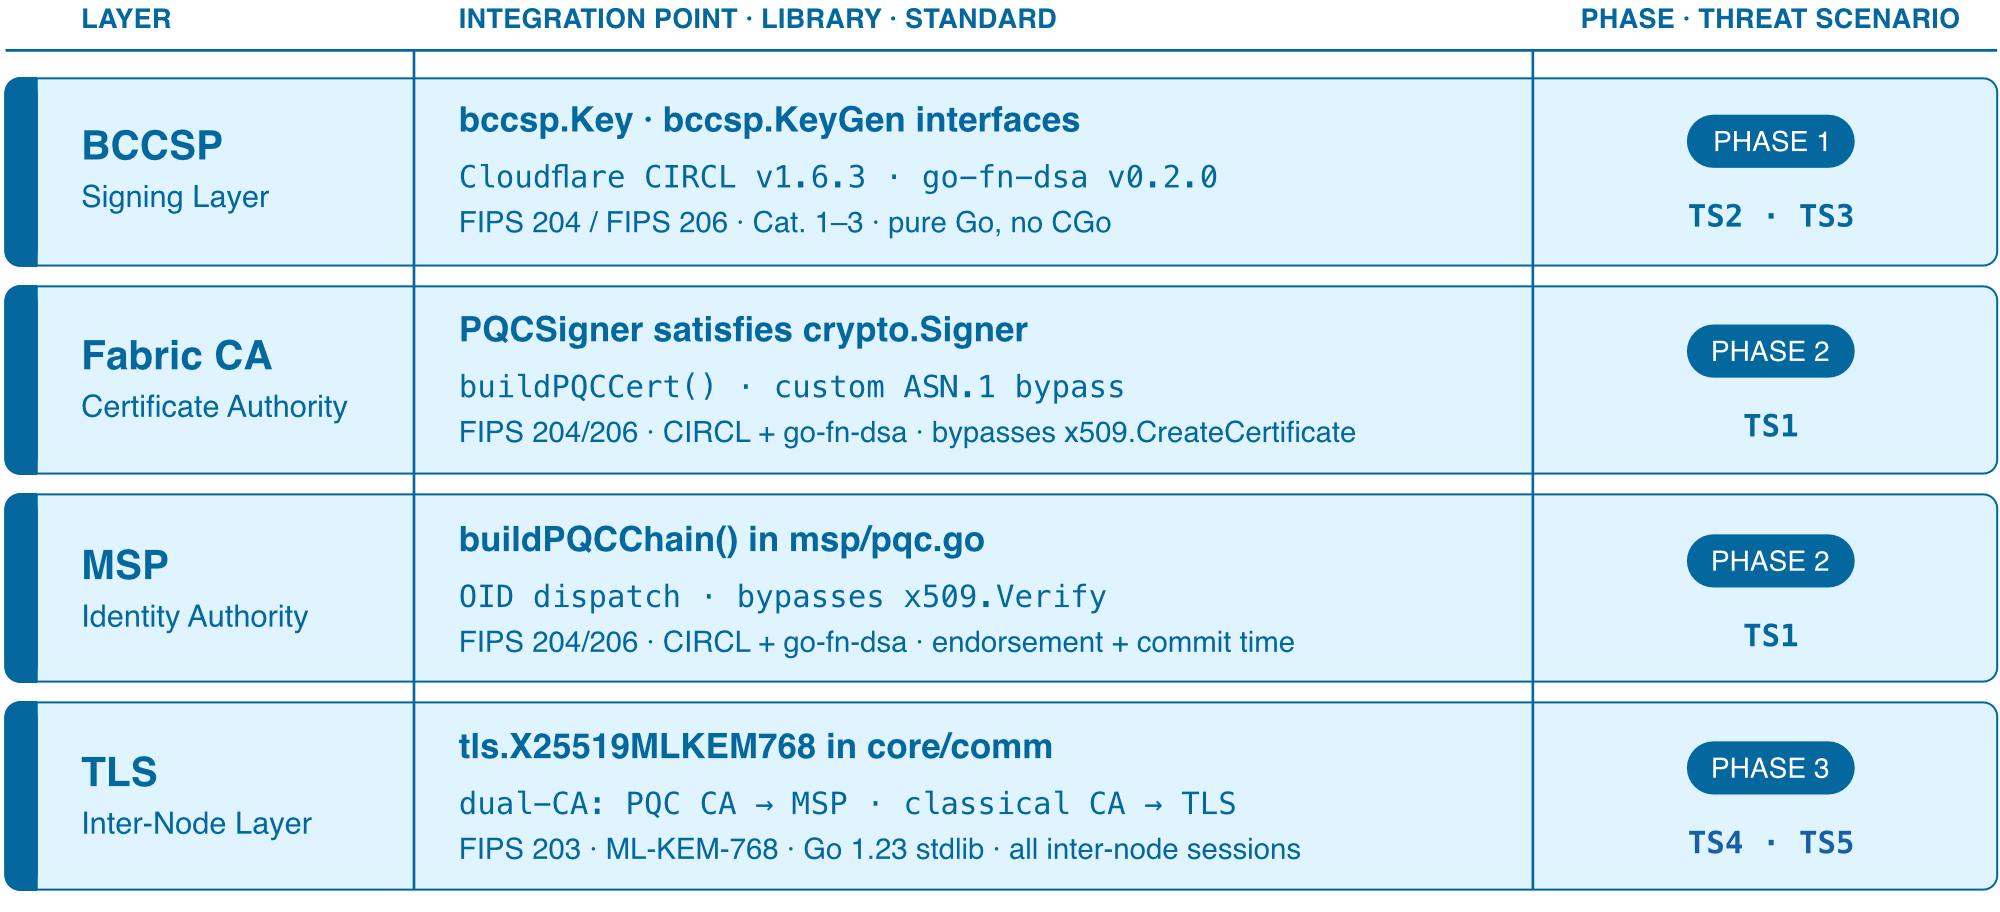
\includegraphics[width=\textwidth]{figures/fig_m2fabric_architecture.png}
\caption{M\textsuperscript{2}Fabric Multilayer Post-Quantum Cryptographic Architecture}
\label{fig:m2fabric_architecture}
\end{figure*}

The BCCSP layer implements Fabric's \textit{bccsp.Key}/\textit{bccsp.KeyGen}
interfaces through the PQC-BCCSP plugin (CIRCL for ML-DSA, \textit{go-fn-dsa}
for FN-DSA, pure Go, no CGo). The Fabric CA layer implements the CFSSL
\textit{crypto.Signer} interface through \textit{PQCSigner} and constructs
post-quantum X.509 certificates via \textit{CreatePQCCertificate()}, which
bypasses \textit{x509.CreateCertificate} through custom ASN.1 encoding because
the standard library rejects post-quantum OIDs. The MSP layer implements
\textit{buildPQCChain()} in \textit{msp/pqc.go}, which dispatches chain
validation on each child's top-level \textit{signatureAlgorithm} OID, performs
full per-link signature verification against the \textit{TBSCertificate},
and enforces validity-period, \textit{keyCertSign}, and AKID/SKID checks,
bypassing \textit{x509.Certificate.Verify}. The TLS layer sets
\textit{tls.X25519MLKEM768} as the preferred key-agreement identifier in
\textit{internal/pkg/comm/}. The certificate-authority layer issues
post-quantum MSP identity certificates that Fabric uses for participant
authentication; the post-quantum hybrid key exchange at the transport
layer is independent of the certificate-authority modifications and is
described in the \textit{TLS Layer Implementation} subsection below.

The four layers correspond to the four categories of cryptographic operation
identified in the threat model. Each is implemented by a self-contained set of
source changes that interact with the others only through existing Fabric
interface contracts. During transaction processing the BCCSP layer is invoked by
peer and orderer to sign transactions, endorsements, and block headers; the
certificate layer is invoked by Fabric CA at enrolment time; the MSP layer is
invoked at endorsement and commit time to validate certificate chains; and the
TLS layer operates continuously for all inter-node communication. These
interactions require the four layers to be mutually consistent: the certificate
format produced by the CA must be compatible with the MSP chain validator;
public keys embedded in certificates must be importable by the BCCSP plugin; and
the algorithm OIDs in the detection table must match those used by the
certificate-generation functions.

\subsubsection{Three-Phase Migration Design}

The implementation is structured in three phases that progressively activate the
four layers, satisfying R8 and enabling per-layer empirical attribution
(\textit{Baseline and Per-Phase Throughput Results} subsection of the
\textit{Experimental Setup and Results} section). We can express the
residual quantum-attack
surface after phase $\phi$ as

\begin{equation}
R(\phi) \;=\; \sum_{i=1}^{5} s_i\,\bigl(1 - c_i(\phi)\bigr),
\label{eq:residual_surface}
\end{equation}

where $s_i>0$ is the severity weight of threat scenario $\mathrm{TS}_i$ and
$c_i(\phi)\in\{0,1\}$ indicates whether $\mathrm{TS}_i$ is closed at the end of
phase $\phi$. The migration design drives $R(\phi)$ monotonically to zero:
$R(0)=\sum_i s_i$ (classical baseline), $R(1)>0$ (TS1 remains open),
$R(2)$ closes TS1--TS3, and $R(3)=0$ once the hybrid-TLS layer closes TS4 and the
TLS component of TS5. Figure~\ref{fig:phase_migration_design} presents this
sequence as a timeline; the red Phase~1 badge marks the open TS1 surface that
motivates the multilayer design.

\begin{figure}[ht]
\centering
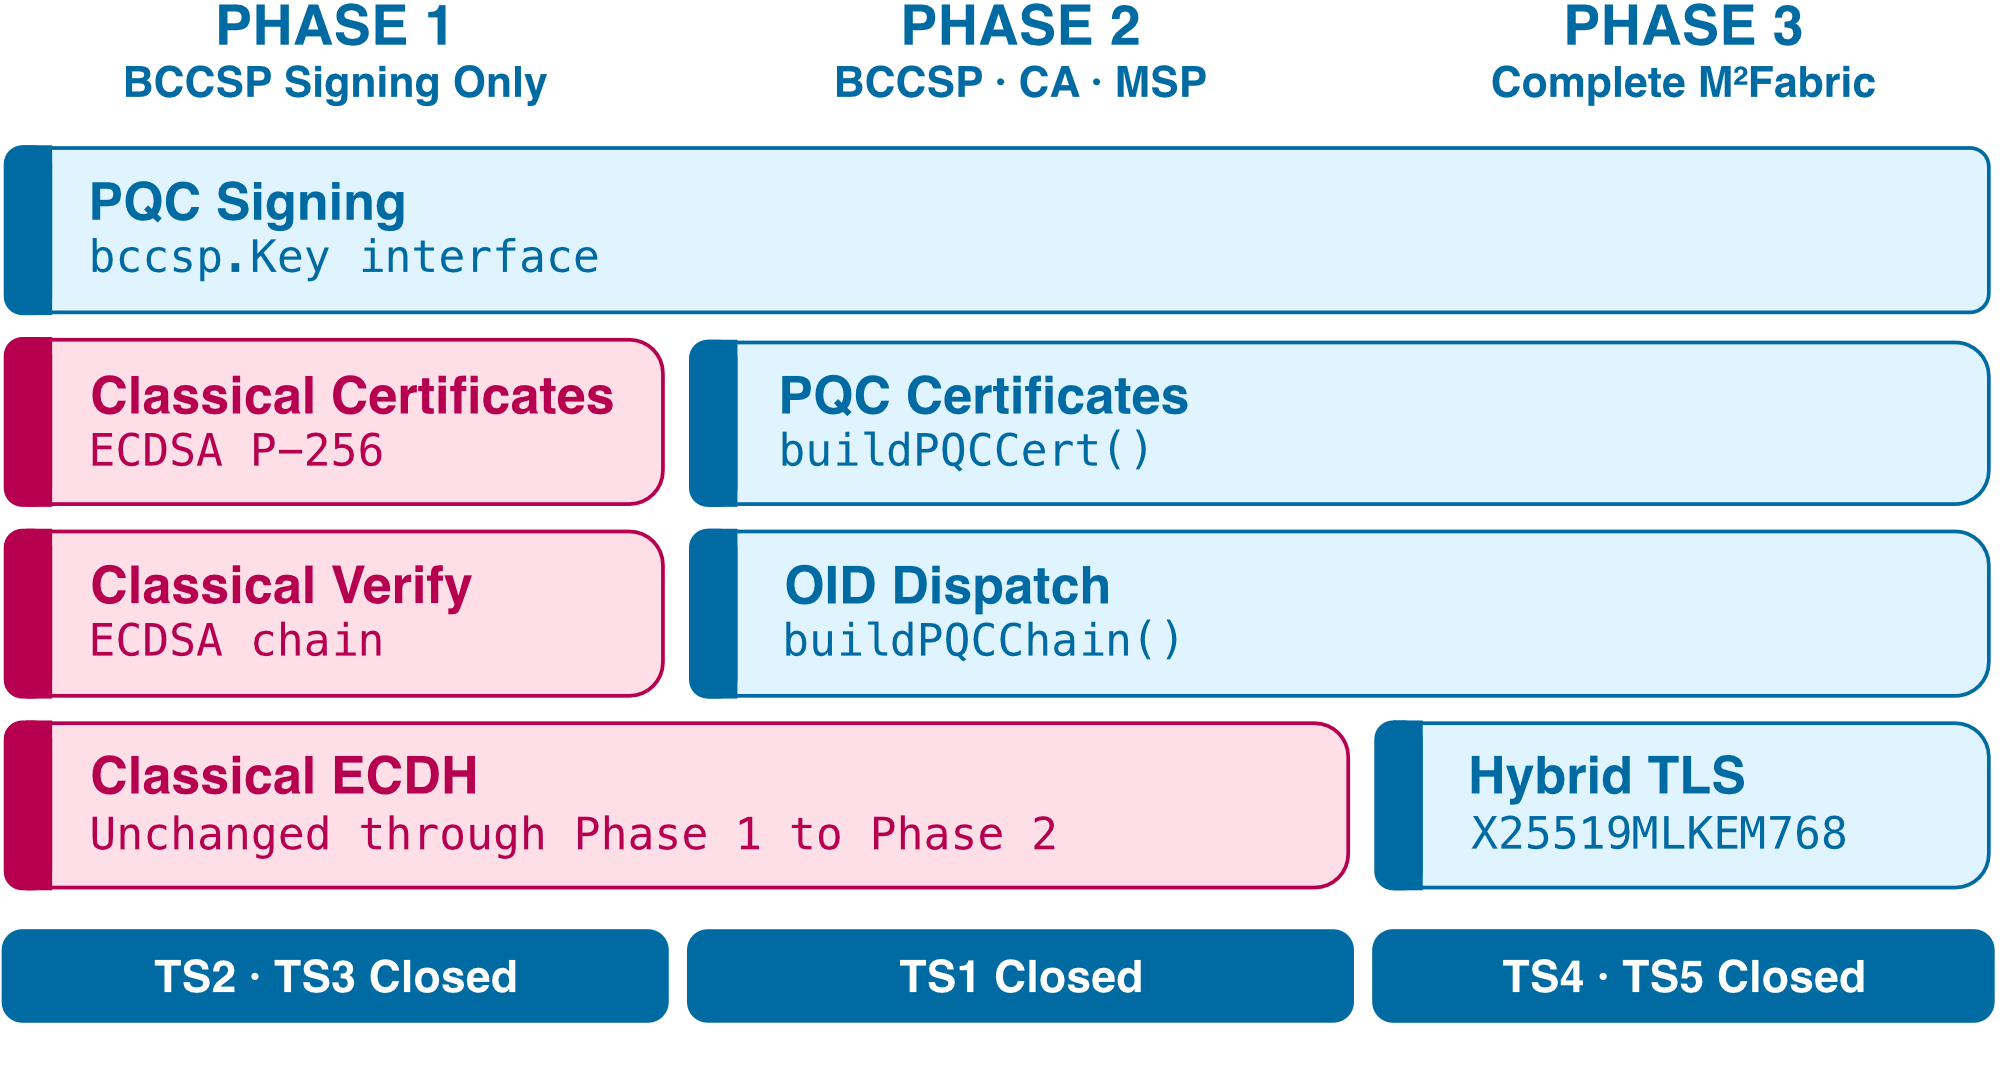
\includegraphics[width=8.6cm]{figures/fig_phase_migration_design.png}
\caption{M\textsuperscript{2}Fabric Migration Sequence}
\label{fig:phase_migration_design}
\end{figure}

\textbf{Phase 1} activates the PQC BCCSP signing layer only: all transaction,
endorsement, block-header, and channel-configuration signatures use the
configured post-quantum algorithm, while certificates and TLS remain classical.
Phase~1 partially addresses TS2 and TS3 (an adversary cannot forge post-quantum
signatures even with a CRQC) but leaves TS1 completely open: because the CA
public keys remain ECDSA, an adversary who recovers the CA private key can still
issue fraudulent post-quantum certificates accepted by the MSP. Phase~1 protects
the signing path but not the certificate trust path.

\textbf{Phase 2} adds the PQC certificate infrastructure: all enrolled
identities receive post-quantum certificates, and MSP validation uses
\textit{buildPQCChain()}. TS1, TS2, and TS3 are all fully addressed. The CA must
be bootstrapped with the \mfabric{} extension, and all identities enrolled under
the classical CA must be re-enrolled to obtain post-quantum credentials.
This is the most operationally significant migration step, requiring all
nodes, clients, and
administrators to obtain new key material and restart, with cross-organisational
coordination in a multi-organisation deployment.

\textbf{Phase 3} adds hybrid TLS key exchange (\textit{X25519MLKEM768}) for all
inter-node connections, constituting the complete deployment. It closes TS4
(TLS session decryption) and the TLS component of TS5 (gossip manipulation),
yielding the fully post-quantum-resistant configuration in which $R(3)=0$.

\subsection{BCCSP Layer Implementation}
\label{sec:method_bccsp}

The Blockchain Cryptographic Service Provider interface, defined in
\textit{bccsp/bccsp.go}, is Fabric's abstraction for cryptographic services
(seven method families: \textit{KeyGen}, \textit{KeyImport}, \textit{GetKey},
\textit{Sign}, \textit{Verify}, \textit{Hash}, \textit{GetHashOpts}); no
component contains algorithm-specific code outside the BCCSP. The
\mfabric{} plugin is grafted into the software backend through a
self-contained PQC wrapper and verifier (\textit{bccsp/sw/pqckey.go}) and
exposed via a separate factory (\textit{bccsp/factory/pqcfactory.go}) that
registers the \textit{PQC} backend without disturbing the classical
backend's call sites.

The plugin implements the full \textit{bccsp.BCCSP} interface for ML-DSA-44,
ML-DSA-65, and FN-DSA-512, instantiated when \textit{core.yaml} specifies
\textit{Default: PQC} with the variant named in the \textit{Algorithm}
field. Key generation invokes CIRCL or \textit{go-fn-dsa} with
\textit{crypto/rand} and stores keys in ASN.1 Distinguished Encoding
Rules (DER) format. ML-DSA signing uses the
pure FIPS~204 mode (full-message with internal SHAKE-256), preserving
FIPS-level domain separation; FN-DSA signing produces a variable-length
NTRU-lattice signature centred on $\sim$666~bytes, which Fabric's unbounded
protobuf signature fields accommodate without serialisation changes.
\textit{KeyImport} inspects the SubjectPublicKeyInfo (SPKI) OID,
deserialising post-quantum key bytes or delegating classical OIDs to
the software BCCSP; \textit{Hash}
and \textit{GetHashOpts} are delegated unconditionally since SHA-256 and
SHA-3 are not replaced.

All Fabric signing paths (peer endorsement, orderer block signing, client
proposal signing) call \textit{Sign} through existing helpers; switching
\textit{Default} from software to \textit{PQC} redirects all signing and
verification, satisfying DP1 and DP4. Algorithm dispatch is table-driven
(a map keyed by algorithm name), so a new algorithm requires only a new
entry, satisfying R5. Private keys are serialised with their algorithm
identifier and type-checked at load to prevent cross-algorithm misuse. The
principal new files are \textit{bccsp/sw/pqckey.go} and
\textit{bccsp/factory/pqcfactory.go} (Table~\ref{tab:impl_scope}); core
PQC primitives live in the external pure-Go \textit{pqc-bccsp} module that
reuses the chain validator's dispatch table (\textit{MSP Identity
Validation} subsection of the \textit{Methodology} section).
Table~\ref{tab:impl_scope} enumerates the files modified or created
across the Fabric v2.5.12 and Fabric CA v1.5.12 source trees. The
``(new)'' annotation marks newly created files, and the ``(delta)''
annotation marks lines added to an existing file.

\begin{table*}[ht]
\centering
\caption[Implementation scope: files modified across Fabric and Fabric CA.]
{Implementation scope of \mfabric{} across Hyperledger Fabric and
Fabric CA.}
\label{tab:impl_scope}
\setlength{\tabcolsep}{3pt}
\footnotesize
\begin{tabular}{p{2.6cm}p{4.5cm}p{7cm}r@{}}
\toprule
\textbf{Repository} & \normalfont\textbf{File} & \textbf{Purpose} & \textbf{Lines of Code} \\
\midrule
\multicolumn{4}{@{}l@{}}{\textit{\textbf{Hyperledger Fabric v2.5.12: BCCSP layer (new)}}} \\
Fabric & bccsp/sw/pqckey.go        & PQC public-key wrapper + SPKI parser + verifier (new) & 90 \\
Fabric & bccsp/factory/pqcfactory.go & PQC backend factory + registration (new) & 206 \\
\addlinespace
\midrule
\multicolumn{4}{@{}l@{}}{\textit{\textbf{Hyperledger Fabric v2.5.12: MSP layer}}} \\
Fabric & msp/pqc.go                & \textit{buildPQCChain()} validator + helpers (new) & 303 \\
Fabric & msp/mspimpl.go            & PQC dispatch hook (delta) & 14 \\
Fabric & msp/pqc\_test.go          & Unit tests for \textit{buildPQCChain} (new) & 252 \\
\addlinespace
\midrule
\multicolumn{4}{@{}l@{}}{\textit{\textbf{Hyperledger Fabric v2.5.12: TLS layer (delta)}}} \\
Fabric & internal/pkg/comm/config.go     & X25519MLKEM768 server preference & 3 \\
Fabric & internal/pkg/comm/server.go     & X25519MLKEM768 gRPC-server preference & 3 \\
Fabric & internal/pkg/comm/connection.go & X25519MLKEM768 client preference & 3 \\
\addlinespace
\midrule
\multicolumn{4}{@{}l@{}}{\textit{\textbf{Hyperledger Fabric v2.5.12: Configuration}}} \\
Fabric & core.yaml                 & PQC BCCSP provider + algorithm keys & 16 \\
Fabric & go.mod                    & CIRCL, go-fn-dsa, pqc-bccsp deps & 6 \\
\addlinespace
\midrule
\multicolumn{4}{@{}l@{}}{\textit{\textbf{Fabric CA v1.5.12: Certificate infrastructure}}} \\
CA & util/pqcsigner.go         & PQCSigner + \textit{CreatePQCCertificate} + key utilities (new) & 729 \\
CA & lib/ca.go                 & PQC key loading + signer selection (delta) & 42 \\
CA & lib/serverenroll.go       & Algorithm detection at enrolment (delta) & 18 \\
CA & cmd/fabric-ca-server/config.go & PQC algorithm config field (delta) & 14 \\
CA & util/csp.go               & PQC dispatch in BCCSP wiring (delta) & 8 \\
CA & go.mod                    & Library dependencies & 6 \\
\midrule
\multicolumn{3}{@{}l@{}}{\textbf{Approximate total new or modified lines of Go}} & \textbf{1{,}713} \\
\bottomrule
\end{tabular}
\end{table*}

\subsection{Certificate Infrastructure Implementation}
\label{sec:method_ca}

The most significant implementation challenge is the incompatibility between
post-quantum OIDs and Go's \textit{crypto/x509} package, which (through
Go~1.24, the version targeted by this work) supports only RSA and ECDSA
signature algorithms and no post-quantum algorithm. Calling \textit{x509.CreateCertificate} with a
post-quantum key, or \textit{x509.Certificate.Verify} on a post-quantum
signature, returns an unsupported-algorithm error. This barrier is why prior
post-quantum Fabric implementations have relied on offline certificate
generation, leaving the live CA's ECDSA signing key active. This is
precisely the gap that creates the TS1 vulnerability. \mfabric{} resolves the barrier through a
custom certificate construction function in Fabric CA and the custom
\textit{buildPQCChain()} validator in the MSP.

\subsubsection{Fabric CA Post-Quantum Extension}

The \mfabric{} extension adds post-quantum issuance to a single Fabric CA
process through three coordinated changes in
\textit{fabric-ca/util/pqcsigner.go}, \textit{fabric-ca/lib/ca.go}, and
\textit{fabric-ca/lib/serverenroll.go}. The first defines the
\textit{CreatePQCCertificate} function that constructs an X.509 v3
certificate manually in ASN.1 DER following RFC~5280~\cite{rfc5280}, with
the SubjectPublicKeyInfo carrying the post-quantum public key under the
NIST OID for ML-DSA-44 (\textit{2.16.840.1.101.3.4.3.17}); FN-DSA-512 uses
the provisional OID \textit{1.3.9999.3.6} from the Open Quantum Safe
experimental arc, slated to be superseded by the finalised FIPS~206 OID
via a single-constant change with a transition-window entry in the
validator's dispatch table to preserve verifiability of certificates
issued under the provisional assignment.

The integration with Fabric CA's signing path is achieved by registering
a global hook with the (forked) CFSSL local signer at package
initialisation time:
\textit{local.SetPQCCertCreator(...)}. When the CFSSL
\textit{local.Signer} is invoked from
\textit{ca.enrollSigner.Sign(req.SignRequest)}, it inspects the
certificate template's public key; if the type is \textit{PQCPublicKey}
or \textit{PQCPublicKeyRaw} (the latter populated from a client-submitted
PQC CSR), the hook dispatches to \textit{CreatePQCCertificate}, otherwise
the standard \textit{crypto/x509} path is used. The assembled TBS is
signed directly with the CA's post-quantum private key through the
\mfabric{} BCCSP plugin; no caller-side pre-hash is applied, since ML-DSA
and FN-DSA perform the FIPS-mandated internal hashing (SHAKE-256 for
FIPS~204, hash-to-point for FIPS~206). The DER output is parseable by
any RFC~5280-conformant implementation. The only differences from a
classical certificate are the two algorithm-identifier OID values and
the key/signature byte lengths, so post-quantum certificates flow through
the existing MSP directory structure and channel-configuration
mechanisms unchanged.

The enrolment handler in \textit{serverenroll.go} contains a
complementary fallback path for the CSR parsing step: when
\textit{x509.ParseCertificateRequest} fails because the CSR carries an
unknown post-quantum OID, the handler invokes
\textit{util.ExtractCNFromCSR} to extract the subject common name
directly from the ASN.1 bytes, allowing the standard policy and
attribute checks to proceed. The CA key-generation subsystem self-signs
a post-quantum root when \textit{csr.key.algo} specifies a post-quantum
algorithm. Through these changes the \mfabric{} Fabric CA binary remains
a drop-in replacement for the standard Fabric CA: the API contract and
endpoint surface are unchanged.

\subsubsection{End-to-End Identity Lifecycle}

Figure~\ref{fig:dual_ca_architecture} traces an MSP identity certificate
through its lifecycle inside \mfabric{}, from the moment a peer, orderer,
or client submits an enrolment request to the moment the certificate is
validated at endorsement or commit. Four phases structure the flow.
In the CA-process phase, the \mfabric{} Fabric CA runs as a single
modified Fabric CA v1.5.12 binary configured with a post-quantum
\textit{csr.key.algo} value (for example, \textit{ml-dsa-44}). In the
issuance phase, the \textit{/enroll} handler in \textit{lib/serverenroll.go}
receives the request, applies the \textit{ExtractCNFromCSR} fallback when
the CSR carries an unknown post-quantum OID, and forwards the validated
request to \textit{ca.enrollSigner.Sign}; the forked CFSSL local signer
then invokes the \textit{PQCCertCreator} hook registered at package
initialisation, dispatching to \textit{CreatePQCCertificate} which
constructs the certificate manually in ASN.1 DER and signs the TBS
through the \mfabric{} BCCSP plugin using the configured post-quantum
algorithm. In the artefact phase, the resulting MSP identity certificate
carries a post-quantum public key (ML-DSA-44, ML-DSA-65, or FN-DSA-512)
under the matching NIST or transitional OID and is committed to the
ledger and to the channel configuration. In the validation phase, every
endorsement and commit triggers \textit{getUniqueValidationChain} in
\textit{mspimpl.go}, which routes post-quantum certificates to
\textit{buildPQCChain} for OID-dispatched chain validation.

This lifecycle is the path Fabric uses for participant identity. The MSP
identity certificate is the artefact Fabric authenticates against in
every transaction, every endorsement-policy evaluation, and every channel
configuration update. The certificate-infrastructure layer of \mfabric{}
is therefore fully post-quantum end-to-end, from CA root self-signing
through runtime chain validation at the committing peer.

\begin{figure}[ht]
\centering
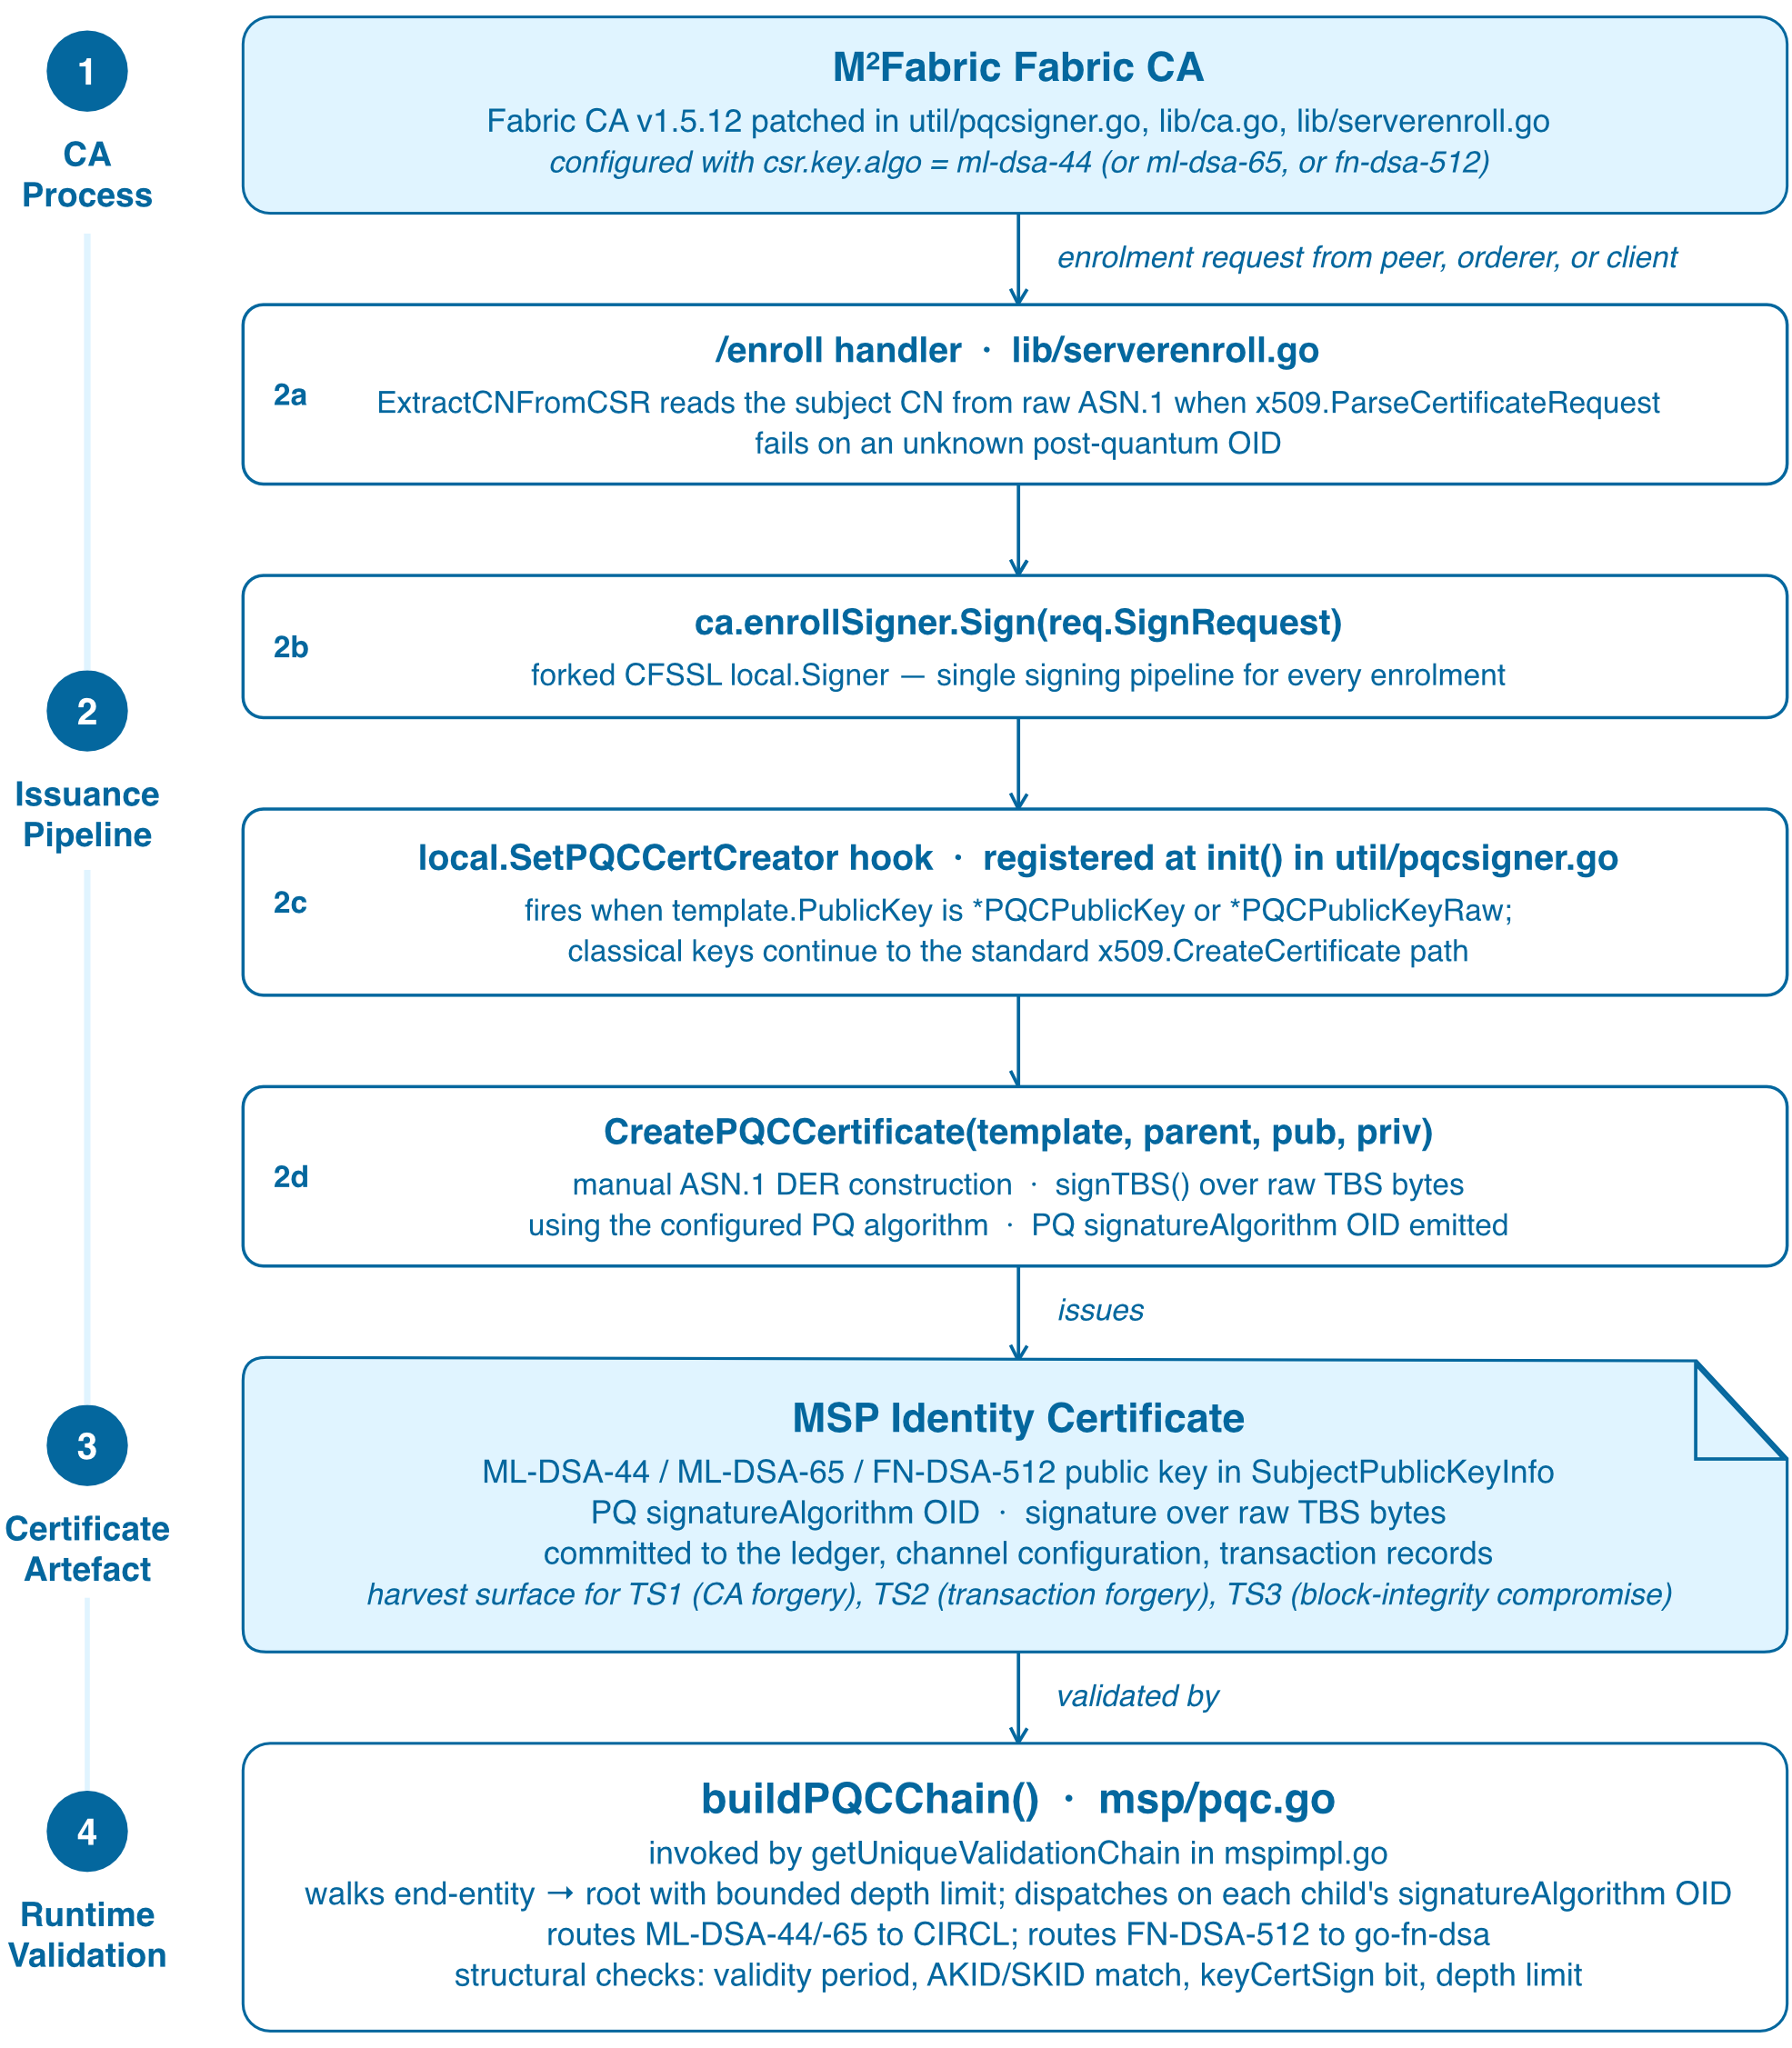
\includegraphics[width=8.6cm]{figures/fig_dual_ca_architecture.png}
\caption[M\textsuperscript{2}Fabric post-quantum identity lifecycle.]
{M\textsuperscript{2}Fabric post-quantum MSP identity certificate
lifecycle, from enrolment to runtime validation.}
\label{fig:dual_ca_architecture}
\end{figure}

The IETF-track composite-signature
construction~\cite{ounsworth2024composite}
(\textit{draft-ietf-lamps-pq-composite-sigs}) provides a future
extensibility path for the same dispatch mechanism, pairing classical and
post-quantum signatures inside a single certificate; the \mfabric{}
dispatch table and \textit{CreatePQCCertificate} construction generalise
directly to that construction once it standardises.

\subsection{MSP Identity Validation: The \textit{buildPQCChain()} Validator}
\label{sec:method_msp}

MSP identity validation requires verifying certificate chains for all
identities in channel transactions, since these chains are what Fabric
uses to authenticate every endorsement, every commit, every channel
configuration update, and every administrative action. The standard MSP
uses Go's \textit{x509.Certificate.Verify}, which is hardcoded to Go's
supported signature set and rejects post-quantum chains on sight, and
the hybrid chains required by the post-quantum lifecycle therefore need
a dedicated validator.
Figure~\ref{fig:buildpqcchain_flowchart} presents the
\textit{buildPQCChain()} control flow. The validator walks the chain
from end-entity to root under a bounded depth limit of ten links and
terminates successfully when it reaches a self-signed certificate that
matches one of the MSP's configured root anchors. At each non-terminal
link, \textit{findIssuerFor} locates the issuer by matching the child's
\textit{RawIssuer} against the Subject DNs of the MSP's intermediate-CA
and root-CA sets, after which \textit{verifyChainLink} runs the per-link
checks. Algorithm dispatch is keyed simultaneously on the child's
\textit{signatureAlgorithm} OID and the issuer's SubjectPublicKeyInfo
(SPKI) OID: classical OIDs on both sides route to Go's
\textit{Certificate.CheckSignatureFrom}, while post-quantum OIDs invoke
the appropriate CIRCL (for ML-DSA) or \textit{go-fn-dsa} (for FN-DSA)
verifier on the child's \textit{RawTBSCertificate}, with no caller-side
pre-hash. A legacy-format fallback re-resolves the dispatch when the
child carries a classical placeholder OID but the issuer's SPKI is
post-quantum, allowing certificates produced before the cert-generator
fix to verify. Any cross-algorithm inconsistency between the resolved
algorithm and the issuer's algorithm is rejected. When the primary
post-quantum verification over the TBS bytes fails, a SHA-256
pre-hash retry preserves migration-window verifiability for credentials
from the pre-fix generator; if that retry also fails the link is
rejected. Hybrid chains mixing classical and post-quantum algorithms
across links are supported to accommodate phased migrations in which the
trust anchor and end-entity certificates can be issued under different
algorithm families.

\begin{figure}[!t]
\centering
\includesvg[inkscapelatex=false,width=\columnwidth]{figures/fig_buildpqcchain_flowchart}
\caption{Control flow of the \textit{buildPQCChain()} certificate-chain validator in \textit{msp/pqc.go}.}
\label{fig:buildpqcchain_flowchart}
\end{figure}

\textit{verifyChainLink} applies five structural checks in order before
signature verification: the issuer's \textit{notBefore}/\textit{notAfter}
validity window; the child's validity window, skipped when the child and
issuer are the same certificate (as occurs at a self-signed root); the
\textit{BasicConstraints.IsCA} flag on the issuer; the
\textit{keyCertSign} bit of the issuer's KeyUsage extension when that
extension is present; and AKID-to-SKID matching when both extensions are
present per RFC~5280~\cite{rfc5280}. The validator is invoked from
\textit{getUniqueValidationChain} whenever a post-quantum certificate or
trust anchor is present; classical-only deployments take the unchanged Go
path, preserving existing MSP semantics. Overhead beyond OID lookup is
one post-quantum verification per identity per block at Op-16, a minor
contributor relative to Op-14 endorsement re-verification. Algorithm
dispatch is registry-keyed for crypto-agility (R5); unknown OIDs fall
through to the classical path.

\subsection{TLS Layer Implementation}
\label{sec:method_tls}

Go~1.24's \textit{crypto/tls} exposes \textit{X25519MLKEM768} as a
\textit{tls.CurveID} constant, performing both X25519 ECDH and ML-KEM-768
encapsulation in the ClientHello and deriving the session key from the
concatenated output. The construction follows the IETF hybrid
framework~\cite{ietf_hybrid_tls} and the
\textit{draft-kwiatkowski-tls-ecdhe-mlkem} codepoint
\textit{0x11EC}~\cite{ietf_x25519mlkem768}. The Phase~3 session key is

\begin{equation}
K_{\mathrm{sess}} \;=\; \mathrm{HKDF}\!\left(K_{\mathrm{X25519}}\;\big\|\;K_{\mathrm{MLKEM}}\right),
\label{eq:hybrid_key}
\end{equation}

which is computationally indistinguishable from a uniformly random key
provided \emph{either} contributing exchange is secure, satisfying R2 and
the NIST transitional guidance~\cite{barker2020transition,bindel2017}.

\mfabric{} sets \textit{CurvePreferences} to
\textit{[tls.X25519MLKEM768, tls.X25519, tls.CurveP256]} in \textit{comm/}
and \textit{internal/}, placing the hybrid first with classical fallbacks
for interoperability with non-upgraded peers. Raft inter-orderer mutual TLS
(Op-12, Op-13) uses the same configuration; Raft log entries are
transport-authenticated, so Phase~3 protects inter-orderer traffic via TLS
rather than per-message signatures. The hybrid key exchange closes TS4 at
the key-agreement path, providing post-quantum confidentiality for every
inter-node session independently of the certificate-infrastructure layer
discussed earlier.

%=====================================================================
\section{Experimental Setup and Results} \label{sec:experimental}
%=====================================================================

\subsection{Test Network Configuration}
\label{sec:exp_testnet}

The test network is two organisations (one peer each) and a single Raft
orderer on a single physical host, isolating cryptographic overhead from
network latency. The same \mfabric{} binary is used for all phases:
Phase~1 enables the PQC BCCSP with bootstrap ECDSA certificates from a
modified Cryptogen; Phase~2 adds Fabric~CA with the post-quantum extensions
and re-enrols all identities to post-quantum certificates; Phase~3 adds
\textit{X25519MLKEM768} to the TLS preference list and restarts all nodes.
The standard Fabric asset-transfer-basic chaincode is deployed without
modification. This topology is the smallest deployable network that
exercises the full transaction lifecycle, the endorsement-policy mechanism
(both organisations signing), and the Raft consensus path, while keeping
the cryptographic signal uncontaminated by WAN latency, since loopback
transport fully exercises ML-KEM-768 encapsulation and decapsulation. The resulting
throughput is an upper bound for the same configuration on a distributed
network.

\subsection{Benchmark Methodology}
\label{sec:exp_benchmethod}

Table~\ref{tab:benchmark_env} summarises the benchmark environment.

\begin{table}[ht]
\centering
\caption{Benchmark environment specification.}
\label{tab:benchmark_env}
\setlength{\tabcolsep}{5pt}
\footnotesize
\begin{tabular}{@{}>{\raggedright\arraybackslash}p{2.7cm}>{\raggedright\arraybackslash}p{5.5cm}@{}}
\toprule
\textbf{Parameter} & \textbf{Value} \\
\midrule
\multicolumn{2}{@{}l@{}}{\textit{Hardware}} \\
Processor      & Intel Core i9-9980HK, 8 cores @ 2.4 GHz (turbo 5.0 GHz) \\
Memory         & 64 GB DDR4 \\
Host OS        & macOS \\
Deployment     & Docker containers, single host \\
\addlinespace
\multicolumn{2}{@{}l@{}}{\textit{Software}} \\
Hyperledger Fabric & v2.5.12 (commit \textit{af0b647}) \\
Fabric CA          & v1.5.12 \\
Hyperledger Caliper & v0.6.0 \\
Go runtime         & 1.24 (binaries pinned to 1.24, the version that supplies \textit{tls.X25519MLKEM768}) \\
PQC libraries      & Cloudflare CIRCL v1.6.3, go-fn-dsa v0.2.0 \\
\addlinespace
\multicolumn{2}{@{}l@{}}{\textit{Network topology}} \\
Organisations  & 2, each with 1 peer node \\
Ordering service & 1 Raft node (Crash Fault Tolerant) \\
Fabric CA instances & 2 (one per organisation) \\
Consensus      & Raft (Crash Fault Tolerant) \\
\addlinespace
\multicolumn{2}{@{}l@{}}{\textit{Channel configuration}} \\
Maximum block size & 500 transactions \\
Block timeout      & 2 seconds \\
Endorsement policy & Any 1 of 2 organisations \\
Chaincode          & Asset transfer (key-value ledger) \\
\addlinespace
\multicolumn{2}{@{}l@{}}{\textit{Benchmark protocol}} \\
Send-rate sweep    & 13 levels: 25, 50, 100, 150, 200, 300, 400, 500, 600, 700, 800, 900, 1000 TPS \\
Runs per config    & 3 independent runs \\
Workload profiles  & Write-heavy (90\% write), mixed (50\% write) \\
\bottomrule
\end{tabular}
\end{table}

The write-heavy workload (90\%/10\%) models a transaction-intensive
supply-chain or financial ledger; the mixed workload (50\%/50\%) models a
general-purpose application; the network is reset to a clean genesis block
before each write-heavy run. Caliper~\cite{caliper2023} sweeps thirteen
target rates from 25 to 1{,}000~TPS, submitting transactions for a fixed
window at each rate. Maximum sustainable throughput is identified as the
plateau-region mean across three runs:

\begin{equation}
\Gamma_{\max} \;=\; \frac{1}{|\mathcal{P}|}\sum_{\rho\in\mathcal{P}}\Gamma_{\mathrm{ach}}(\rho),
\quad
\mathcal{P}=\Bigl\{\rho:\bigl|\tfrac{d\Gamma_{\mathrm{ach}}}{d\rho}\bigr|\le\varepsilon\Bigr\},
\label{eq:plateau}
\end{equation}

where $\mathcal{P}$ is the set of send rates over which achieved throughput
is stationary below a small saturation threshold $\varepsilon$. Four metrics
are reported: $\Gamma_{\max}$ (TPS), saturation latency (s), ledger storage
(MB/peer, measured directly after each run), and block propagation rate
(blocks/s from Prometheus over a 30-minute window).

\subsection{Verification and Correctness Assurance}
\label{sec:exp_verify}

\subsubsection{Cryptographic Primitive Verification}

ML-DSA primitive correctness rests on Cloudflare CIRCL's upstream NIST
ACVP test-vector coverage for FIPS~204; the \textit{pqc-bccsp} dispatch
layer adds no algorithmic logic, so the integration does not re-run ACVP
vectors locally. \mfabric{}'s own suite verifies plugin routing: unit tests
in \textit{msp/pqc\_test.go} generate fresh ML-DSA-44 and ML-DSA-65
keypairs through the plugin, sign and verify \textit{TBSCertificate} bytes
via the live chain validator, and confirm that valid signatures verify and
tampered ones do not. NIST ACVP vectors are not available for FN-DSA
through \textit{go-fn-dsa} v0.2.0 at implementation time, so FN-DSA
correctness is verified through round-trip integration tests on a real
X.509 \textit{TBSCertificate} (\textit{TestBuildPQCChain\_ValidChain/FNDSA512})
and tampered-signature rejection
(\textit{TestBuildPQCChain\_TamperedSignature/FNDSA512}).

\subsubsection{Interface Compliance and End-to-End Verification}

The plugin satisfies the
\textit{Sign}/\textit{Verify}/\textit{KeyImport}/\textit{GetKey} contracts
structurally, by registering through the existing factory machinery and
running through unmodified call sites in peer, orderer, and client SDK.
The table-driven \textit{TestBuildPQCChain\_ValidChain} suite sweeps
ML-DSA-44, ML-DSA-65, and FN-DSA-512, confirming key-generation,
keystore-roundtrip, and error-path semantics (tampered signatures,
expired certificates, unknown issuers, untrusted self-signed). End-to-end
execution covers all five lifecycle phases in each of the three deployment
phases for all three algorithms; all transactions succeed with zero
failures. Verification also confirms correct dispatch inside the MSP:
post-quantum certificates flow through \textit{buildPQCChain()} via
\textit{getUniqueValidationChain}, while classical chains (such as those
loaded for migration-window trust anchors) continue to take the unchanged
Go standard-library path, with no cross-contamination between the two.

\subsubsection{Verification Results Summary}
\label{sec:exp_verifysummary}

Four quantitative properties are established.
\emph{Integration coverage} across the four cryptographic layers that
participate in Hyperledger Fabric's security model, namely BCCSP signing,
MSP certificate infrastructure, MSP identity validation, and the TLS
inter-node session-key path:

\begin{equation}
\delta_{\mfabric} = 
\frac{|\{\text{post-quantum deployed}\}|}
{|\{\text{ECDLP-vulnerable identified}\}|}
= \frac{4}{4} = 1,
\label{eq:integration_coverage}
\end{equation}

with no prior published integration achieving
$\delta=1$~\cite{holcomb2021, hu2025prototype, abbas2025}.
\emph{Signature-size amplification}
$\alpha_{\mathrm{sig}}(\mathrm{alg})=|\sigma_{\mathrm{alg}}|/|\sigma_{\mathrm{ECDSA}}|$
relative to the 72-byte ECDSA baseline gives 9.3, 33.6, and 46.0 for
FN-DSA-512, ML-DSA-44, and ML-DSA-65 respectively, propagating into the
per-block payload analysed in the \textit{Consolidated Analysis and
Performance Models} subsection of the \textit{Experimental Setup and
Results} section.
\emph{Hybrid TLS session-key security} is established
by~(\ref{eq:hybrid_key}): $K_{\mathrm{sess}}$ is secure as long as either
contributing exchange is secure. \emph{BCCSP correctness} was confirmed by
zero verification failures across all ACVP, round-trip, interface, and
end-to-end tests; with $n=27$ benchmark runs per workload across nine
algorithm-phase combinations and $\approx 1.7\times 10^{5}$ committed
post-quantum transactions, the Clopper-Pearson 95\% upper bound on the
per-transaction failure probability is $p<1.8\times 10^{-5}$.

\subsection{Baseline and Per-Phase Throughput Results}
\label{sec:exp_results}

\subsubsection{ECDSA P-256 Baseline}

The ECDSA P-256 baseline (Table~\ref{tab:ecdsa_baseline}) achieves
\textbf{275.3~transactions per second (TPS)} (standard deviation 1.35)
write-heavy and \textbf{344.2~TPS} (standard deviation 1.93) mixed, with
the saturation knee at 200--300~TPS write-heavy and 300--400~TPS mixed
and below-saturation latency of 0.07--0.22~seconds. These
figures are consistent with prior characterisations of standard
Fabric~\cite{androulaki2018, baliga2018performance, kuzlu2021performance, nasir2018}
after accounting for hardware and topology differences.

\begin{table}[ht]
\centering
\caption{ECDSA P-256 baseline results.}
\label{tab:ecdsa_baseline}
\setlength{\tabcolsep}{3.5pt}
\begin{tabular}{@{}p{2.3cm}cccc@{}}
\toprule
\textbf{Workload} & \textbf{ Maximum } & \textbf{Standard} &
\textbf{ Average } & \textbf{Ledger} \\
\textbf{} & \textbf{TPS} & \textbf{ Deviation } &
\textbf{Latency} & \textbf{ Per Peer } \\
\midrule
Write (90\% write) & 275.3 & 1.35 & 0.18~s & 1{,}690~MB  \\
Mixed (50\% write)       & 344.2 & 1.93 & 0.11~s & 3{,}266~MB \\
\bottomrule
\end{tabular}
\end{table}

\subsubsection{Phase 1: BCCSP Post-Quantum Signing}

Phase~1 replaces ECDSA signing at the BCCSP layer while leaving certificates
and TLS unchanged, isolating the signature-algorithm impact.
Figure~\ref{fig:phase1_write} shows throughput-versus-send-rate curves
(write-heavy workload; one-standard-deviation envelope across three runs);
the mixed-workload curves follow the same qualitative shape.

\begin{figure}[t]
\centering
\includesvg[inkscapelatex=false,width=\columnwidth]{figures/fig_phase1_write}
\caption{Phase~1 throughput versus target send rate, write-heavy workload.}
\label{fig:phase1_write}
\end{figure}

All algorithms follow the same sub-knee saturation profile as ECDSA,
confirming negligible sub-saturation overhead; above the knee each plateau
sits below the ECDSA ceiling in proportion to signature size
(Table~\ref{tab:phase1_results}). The write-heavy ML-DSA-65/ML-DSA-44
$\sim 1.8$~TPS gap is within ML-DSA-65's standard deviation of 6.55~TPS (the study's
largest, traced to a single transient at 700~TPS); the mixed-workload
ordering converges to the headline FN-DSA-512 $>$ ML-DSA-44 $>$ ML-DSA-65.
Plateau latencies are 0.18--0.20~s, indistinguishable from baseline.

\begin{table}[t]
\centering
\caption{Phase~1 throughput results.}
\label{tab:phase1_results}
\footnotesize

\resizebox{\columnwidth}{!}{%
\begin{tabular}{@{}lrrrr@{}}
\toprule
\textbf{Algorithm} &
\multicolumn{2}{c}{\textbf{Write-heavy}} &
\multicolumn{2}{c}{\textbf{Mixed}} \\
\cmidrule(lr){2-3}\cmidrule(lr){4-5}
& \textbf{TPS} & \textbf{$\Delta$} &
  \textbf{TPS} & \textbf{$\Delta$} \\
\midrule
ECDSA P-256 & 275.3 (1.35) & ref.     & 344.2 (1.93) & ref. \\
FN-DSA-512  & 270.7 (2.28) & $-1.7\%$ & 338.2 (0.48) & $-1.7\%$ \\
ML-DSA-44   & 263.8 (2.78) & $-4.2\%$ & 339.2 (1.50) & $-1.4\%$ \\
ML-DSA-65   & 265.6 (6.55) & $-3.5\%$ & 330.0 (2.06) & $-4.1\%$ \\
\bottomrule
\end{tabular}%
}

\end{table}

In Table~\ref{tab:phase1_results}, the TPS column gives the mean throughput
across three runs with the per-run standard deviation in parentheses, and
the $\Delta$ column gives the signed percentage change relative to the
ECDSA P-256 baseline (which serves as the reference row).

\subsubsection{Phase 2: Post-Quantum Certificate Infrastructure}

Phase~2 adds post-quantum X.509 infrastructure: the CA issues
post-quantum-signed certificates and \textit{buildPQCChain()} validates them
at Op-16 (the committing-peer chain re-validation, run for every
endorsement signature in every block). Figure~\ref{fig:phase2_throughput}
and Table~\ref{tab:phase2_results} report the results. The certificate
layer introduces substantially larger reductions than Phase~1 for the
ML-DSA family: FN-DSA-512 declines by 3.3\%/3.2\% (write/mixed) from the
1.7\% Phase~1 penalty, reflecting per-endorsement SPKI cost; ML-DSA-44 by
9.9\%/8.9\%; and ML-DSA-65 by 18.1\%/13.0\%, which is the largest
single-phase impact measured.

\begin{figure*}[ht]
\centering
\includesvg[inkscapelatex=false,width=\textwidth]{figures/fig_phase2_throughput}
\caption{Phase~2 maximum sustainable throughput versus ECDSA P-256 baseline, both workloads.}
\label{fig:phase2_throughput}
\end{figure*}

\begin{table}[!t]
\centering
\caption{Phase~2 throughput results.}
\label{tab:phase2_results}
\footnotesize

\resizebox{\columnwidth}{!}{%
\begin{tabular}{@{}lrrrrr@{}}
\toprule
\textbf{Algorithm} &
\multicolumn{2}{c}{\textbf{Write-heavy}} &
\multicolumn{2}{c}{\textbf{Mixed}} &
\textbf{Latency} \\
\cmidrule(lr){2-3}\cmidrule(lr){4-5}
& \textbf{TPS} & \textbf{$\Delta$} &
  \textbf{TPS} & \textbf{$\Delta$} & \\
\midrule
ECDSA P-256 & 275.3 (1.35) & ref.     & 344.2 (1.93) & ref.     & 0.18 s \\
FN-DSA-512  & 266.1 (0.35) & $-3.3\%$ & 333.2 (0.64) & $-3.2\%$ & 1.71 s \\
ML-DSA-44   & 247.9 (0.78) & $-9.9\%$ & 313.5 (2.14) & $-8.9\%$ & 5.47 s \\
ML-DSA-65   & 225.4 (0.44) & $-18.1\%$ & 299.5 (0.53) & $-13.0\%$ & 10.20 s \\
\bottomrule
\end{tabular}%
}
\end{table}

The TPS column gives the mean across three runs with the standard
deviation in parentheses, the $\Delta$ column gives the signed
percentage change relative to ECDSA P-256, and the Latency column gives
the mean transaction latency in the write-heavy plateau region.

The dominant Phase~2 effect is not throughput reduction but certificate-processing
latency (Figure~\ref{fig:latency_phase}). Phase~1 latencies are indistinguishable
from the 0.18-s ECDSA baseline; the Phase~2 transition produces a qualitative
jump to 1.71~s for FN-DSA-512 (9.5$\times$), 5.47~s for ML-DSA-44 (30$\times$),
and 10.20~s for ML-DSA-65 (57$\times$). This reflects the Op-16
bottleneck~\cite{thakkar2018}: a 500-transaction write-heavy block carries up to
500 chain validations, each over an SPKI of 897, 1{,}312, or 1{,}952~bytes
respectively (versus 65 for ECDSA). Mixed-workload latencies are far lower
(0.14, 0.18, 0.77~s) because fewer write transactions per unit time mean fewer
certificates per block.

\begin{figure}[!t]
\centering
\includesvg[inkscapelatex=false,width=0.95\columnwidth]{figures/fig_latency_phase}
\caption{Average transaction latency at saturation by algorithm and phase, write-heavy workload.}
\label{fig:latency_phase}
\end{figure}


\subsubsection{Phase 3: Complete \texorpdfstring{M\textsuperscript{2}Fabric}{M2Fabric} Deployment}

Phase~3 activates hybrid TLS (\textit{X25519MLKEM768}) for all inter-node
connections, completing the deployment. Figure~\ref{fig:phase3_throughput} and
Table~\ref{tab:phase3_results} present the results. FN-DSA-512 achieves 265.5~TPS
write-heavy and 332.7~TPS mixed ($-3.5\%$, $-3.3\%$); ML-DSA-44 achieves 245.2
and 317.0~TPS ($-10.9\%$, $-7.9\%$); ML-DSA-65 achieves 225.8 and 301.1~TPS
($-18.0\%$, $-12.5\%$).

\begin{figure*}[ht]
\centering
\includesvg[inkscapelatex=false,width=\textwidth]{figures/fig_phase3_throughput}
\caption{Phase~3 complete \mfabric{} deployment throughput versus ECDSA P-256 baseline, both workloads.}
\label{fig:phase3_throughput}
\end{figure*}

\begin{table}[t]
\centering
\caption{Phase~3 throughput results.}
\label{tab:phase3_results}
\footnotesize
\resizebox{\columnwidth}{!}{%
\begin{tabular}{@{}lrrrrr@{}}
\toprule
\textbf{Algorithm} &
\multicolumn{2}{c}{\textbf{Write-heavy}} &
\multicolumn{2}{c}{\textbf{Mixed}} &
\textbf{Latency} \\
\cmidrule(lr){2-3}\cmidrule(lr){4-5}
& \textbf{TPS} & \textbf{$\Delta$} &
  \textbf{TPS} & \textbf{$\Delta$} & \\
\midrule
ECDSA P-256 & 275.3 (1.35) & ref. &
344.2 (1.93) & ref. & 0.18s \\
FN-DSA-512  & 265.5 (1.42) & $-3.5\%$ &
332.7 (4.12) & $-3.3\%$ & 1.80s \\
ML-DSA-44   & 245.2 (0.73) & $-10.9\%$ &
317.0 (2.14) & $-7.9\%$ & 5.49s \\
ML-DSA-65   & 225.8 (2.09) & $-18.0\%$ &
301.1 (2.88) & $-12.5\%$ & 10.52s \\
\bottomrule
\end{tabular}}
\end{table}

The TPS column gives the mean across three runs with the standard
deviation in parentheses, the $\Delta$ column gives the signed
percentage change relative to ECDSA P-256, and the Latency column gives
the mean transaction latency in the write-heavy plateau region.

Phase~2-to-Phase~3 changes are small, span zero, and lie within each Phase~3
standard-deviation envelope: hybrid TLS contributes a per-transaction overhead
below the detection threshold of the $n=3$ design, as expected when
connection-level key-exchange cost amortises across many transactions per TLS
session.

\subsection{Consolidated Analysis and Performance Models}
\label{sec:res_consolidated}

Figure~\ref{fig:phase_progression} traces the per-phase throughput for each
algorithm; Table~\ref{tab:phase_attribution} attributes the reductions. For
FN-DSA-512 the 3.5\% write-heavy total splits roughly evenly between
Phases~1 and~2; for ML-DSA-44 and ML-DSA-65 the certificate layer dominates
(5.7 and 14.6 percentage points respectively), while Phase~3 TLS
contributes under 0.2~percentage points in every case. The dominant determinant is the
per-endorsement payload (2{,}611/6{,}546/8{,}964 bytes for
FN-DSA-512/ML-DSA-44/ML-DSA-65 versus 641 bytes for the ECDSA P-256
baseline), applied to every endorsement in every block, independently
corroborating the PQFabric finding~\cite{holcomb2021}. The attribution table reports absolute TPS
together with the contribution of each phase to the total reduction from
the ECDSA P-256 baseline; the Phase~3 column reports the change from
Phase~2 to Phase~3, which isolates the hybrid TLS overhead.

\begin{figure*}[ht]
\centering
\includesvg[inkscapelatex=false,width=\textwidth]{figures/fig_phase_progression}
\caption{Phase-by-phase throughput progression.}
\label{fig:phase_progression}
\end{figure*}

\begin{table}[!t]
\centering
\caption{Phase-by-phase throughput attribution.}
\label{tab:phase_attribution}
\footnotesize
\resizebox{\columnwidth}{!}{%
\begin{tabular}{@{}lcrrrrr@{}}
\toprule
\textbf{Algorithm} & \textbf{Workload} &
\textbf{ECDSA} & \textbf{Phase 1} & \textbf{Phase 2} &
\textbf{Phase 3} & \textbf{Total $\Delta$} \\
\midrule
\multirow{2}{*}{FN-DSA-512}
  & Write & 275.3 & 270.7 ($-1.7\%$) & 266.1 ($-1.6\%$) & 265.5 ($-0.2\%$) & $-3.5\%$ \\
  & Mixed & 344.2 & 338.2 ($-1.7\%$) & 333.2 ($-1.5\%$) & 332.7 ($-0.2\%$) & $-3.3\%$ \\
\addlinespace
\multirow{2}{*}{ML-DSA-44}
  & Write & 275.3 & 263.8 ($-4.2\%$) & 247.9 ($-5.7\%$) & 245.2 ($-1.0\%$) & $-10.9\%$ \\
  & Mixed & 344.2 & 339.2 ($-1.4\%$) & 313.5 ($-7.5\%$) & 317.0 ($+1.1\%$) & $-7.9\%$ \\
\addlinespace
\multirow{2}{*}{ML-DSA-65}
  & Write & 275.3 & 265.6 ($-3.5\%$) & 225.4 ($-14.6\%$) & 225.8 ($+0.2\%$) & $-18.0\%$ \\
  & Mixed & 344.2 & 330.0 ($-4.1\%$) & 299.5 ($-8.9\%$) & 301.1 ($+0.5\%$) & $-12.5\%$ \\
\bottomrule
\end{tabular}%
}

\end{table}

\subsubsection{Throughput Degradation, Latency, and Storage Models}

The attribution data admit a multiplicative decomposition. Letting
$\delta_p$ denote the per-phase fractional reduction, the Phase~3 throughput is
$\Gamma_{\mathrm{Ph3}} = \Gamma_{\mathrm{ECDSA}}\prod_{p=1}^{3}(1-\delta_p)$,
with the additive approximation $\delta_{\mathrm{total}}\approx
\delta_1+\delta_2+\delta_3$ exact to three decimals for FN-DSA-512
($\max\delta_p=0.017$) and accurate to 0.3~percentage points for ML-DSA-65
($\delta_2=0.146$). Statistically, throughput means are reported with 95\%
Student-$t$ intervals using $t_{0.025,2}=4.303$; adjacent-algorithm
intervals are non-overlapping for the headline write-heavy comparisons.
The ordering FN-DSA-512 $>$ ML-DSA-44 $>$ ML-DSA-65 is additionally robust
to a non-parametric bootstrap ($10^4$ resamples, order-preserving) and to
very large inter-algorithm effect sizes (Cohen's $d\approx 18$ and
$\approx 12$ against the conventional ``large'' threshold of 0.8). Only
small-effect comparisons (notably hybrid TLS) are underpowered;
$n\geq 5$ with analysis-of-variance is recommended for those.

The Phase~2 write latencies follow from the certificate-validation
bottleneck at Op-16. The per-block validation overhead introduced by
Phase~2 relative to Phase~1 is
$\Delta t_{\mathrm{block}} = T_b\bar{e}[\tau_{\mathrm{cert}}(\mathrm{alg})
-\tau_{\mathrm{cert}}(\mathrm{ECDSA})]$,
which dominates saturation latency under the binding-constraint regime.
The empirical $\tau_{\mathrm{cert}}$ scales super-linearly with SPKI size: a
power-law fit $\tau_{\mathrm{cert}}\propto|\mathit{pk}|^{\beta}$ gives
$\beta\approx 2.30$, so doubling the public-key size approximately
quintuples per-certificate validation time.

Ledger storage results in Table~\ref{tab:storage_results} confirm that
signature size is a second-order contributor: incremental storage
$\Delta S = N_{\mathrm{tx}}\bar{e}(|\sigma_{\mathrm{alg}}|-|\sigma_{\mathrm{ECDSA}}|)$
gives $\sim$60~MB for FN-DSA-512 at $N_{\mathrm{tx}}\approx 10^5$,
consistent with the measured 0.99$\times$ write-heavy multiplier. All three
post-quantum algorithms produce write-heavy ledgers within 4\% of the
1{,}690~MB ECDSA baseline. The mixed-workload figures are cumulative
across sequential runs without intervening network reset; the 0.86$\times$
ML-DSA-44 multiplier reflects fewer committed blocks at reduced
throughput, not a per-transaction saving. In Table~\ref{tab:storage_results},
both workloads report the mean per-peer ledger size across three
benchmark runs, with the Ratio column expressing each post-quantum value
as a fraction of the ECDSA P-256 reference for the same workload.
\begin{table}[t]
\centering
\caption{Ledger storage per peer at benchmark conclusion.}
\label{tab:storage_results}
\footnotesize
\setlength{\tabcolsep}{4pt}
\begin{tabular}{@{}lrrrr@{}}
\toprule
\textbf{Algorithm} &
\multicolumn{2}{c}{\textbf{Write-heavy}} &
\multicolumn{2}{c}{\textbf{Mixed}} \\
\cmidrule(lr){2-3}\cmidrule(lr){4-5}
& \textbf{MB} & \textbf{Ratio} & \textbf{MB} & \textbf{Ratio} \\
\midrule
ECDSA P-256 & 1{,}690 & ref.\           & 3{,}266 & ref.\          \\
FN-DSA-512  & 1{,}669 & 0.99$\times$    & 4{,}477 & 1.37$\times$   \\
ML-DSA-44   & 1{,}633 & 0.97$\times$    & 2{,}822 & 0.86$\times$   \\
ML-DSA-65   & 1{,}679 & 0.99$\times$    & 4{,}391 & 1.34$\times$   \\
\bottomrule
\end{tabular}
\end{table}
Table~\ref{tab:block_prop} presents block propagation metrics from
sustained-load Prometheus measurements, with values reported as means
across runs where multiple measurements are available. All post-quantum
configurations achieve 9.5 to 9.8~blocks per second in the mixed workload
and 17.4 to 18.4~blocks per second in the write-heavy workload. Average
block processing time is uniformly $\sim$1.0 to 1.1~milliseconds for all
configurations except the ML-DSA-44 mixed measurement, which exhibits
high variance from a warm-up transient in one run. The $\sim$1~millisecond
per-block figure confirms that the Phase~2 and Phase~3 reductions are
driven by certificate-validation overhead at the committing peer rather
than by gossip propagation or orderer latency.

\begin{table}[t]
\centering
\caption{Block propagation metrics by algorithm and workload.}
\label{tab:block_prop}
\footnotesize

\resizebox{\columnwidth}{!}{%
\begin{tabular}{@{}llrr@{}}
\toprule
\textbf{Configuration} & \textbf{Workload} &
\textbf{Blocks/s} & \textbf{Processing Time} \\
\midrule
ECDSA P-256 & Mixed  & 5.04  & 1.13~ms \\
FN-DSA-512  & Write  & 18.19 & 1.02~ms \\
FN-DSA-512  & Mixed  & 9.69  & 1.06~ms \\
ML-DSA-44   & Write  & 17.94 & 1.27~ms \\
ML-DSA-44   & Mixed  & 9.74  & 1.04~ms \\
ML-DSA-65   & Write  & 18.03 & 1.02~ms \\
ML-DSA-65   & Mixed  & 9.51  & 1.07~ms \\
\bottomrule
\end{tabular}%
}

\end{table}

\subsection{Algorithm Selection Guidance}
\label{sec:res_selection}

The phase attribution confirms the cost-model prediction
(Eq.~\ref{eq:selection_cost}): per-endorsement payload size, not signing
speed, is the dominant determinant. FN-DSA-512 delivers the highest
end-to-end throughput despite signing $\sim$53\% more slowly than ML-DSA-44
in microbenchmarks, because its smaller signature and public key give a far
smaller per-endorsement payload. Table~\ref{tab:selection_matrix}
consolidates the selection matrix. The throughput and latency figures
are the Phase~3 results from Table~\ref{tab:phase3_results} and
Figure~\ref{fig:latency_phase}. Security categories follow NIST FIPS~204
(finalised in 2024) and the FIPS~206 Initial Public Draft (2025). The
$\Delta_{\mathrm{ECDSA}}$ column gives the throughput change relative to
the ECDSA P-256 baselines of 275.3~TPS write-heavy and 344.2~TPS mixed,
and the latency multiplier $L/L_{\mathrm{ECDSA}}$ divides the Phase~3
write-heavy latency by the 0.18~second ECDSA reference.

\begin{table*}[ht]
\centering
\caption{Algorithm selection matrix.}
\label{tab:selection_matrix}
\setlength{\tabcolsep}{3pt}
\footnotesize
\begin{tabular}{@{}lcrrrrcp{7.5cm}@{}}
\toprule
\textbf{Algorithm} & \textbf{Security Category} &
\multicolumn{2}{c}{\textbf{Write-heavy}} &
\multicolumn{2}{c}{\textbf{Mixed}} &
\textbf{$L/L_{\mathrm{ECDSA}}$} &
\textbf{Recommendation} \\
\cmidrule(lr){3-4}\cmidrule(lr){5-6}
& & \textbf{TPS} & \textbf{$\Delta_{\mathrm{ECDSA}}$} &
\textbf{TPS} & \textbf{$\Delta_{\mathrm{ECDSA}}$} & & \\
\midrule
FN-DSA-512 & 1 & 265.5 & $-3.5\%$  & 332.7 & $-3.3\%$  & $10\times$  & Primary: lowest overhead; recommended for throughput-sensitive deployments and early-transition pilots \\
ML-DSA-44  & 2 & 245.2 & $-10.9\%$ & 317.0 & $-7.9\%$  & $30\times$  & Balanced: NIST first-choice signature; recommended where Category~2 assurance is mandated and $\sim$11\% reduction is acceptable \\
ML-DSA-65  & 3 & 225.8 & $-18.0\%$ & 301.1 & $-12.5\%$ & $58\times$  & High-assurance: recommended only where Category~3 is mandated; 18\% reduction and tenfold latency increase must be acknowledged in the deployment design \\
\bottomrule
\end{tabular}
\end{table*}

\subsection{Security Analysis of the Implementation}
\label{sec:res_security}

The security rests on three foundations: the security of the post-quantum
algorithms (established by NIST's six-year standardisation
process~\cite{alagic2022nist}; no polynomial-time quantum algorithm is known for
the underlying Module LWE or NTRU/SIS problems), the correctness of the
implementation (established by the verification reported in the
\textit{Verification and Correctness Assurance} subsection of the
\textit{Experimental Setup and Results} section), and the integrity of
the integration design (which preserves the existing Fabric
security model: the BCCSP contract is satisfied exactly, MSP policy evaluation is
unchanged, the TLS configuration is a subset of Go's option space, and CA-issued
certificates follow the RFC~5280 structure).

The custom code paths added above the primitive layer are not covered by upstream
review and warrant explicit identification of residual attack surface. Four
classes of concern apply. \textit{Malformed-certificate handling}: the custom
ASN.1 parser in \textit{buildPQCChain()} operates on attacker-controlled input;
it rejects parsing failures by error-return rather than panic, but
positive evidence of robustness requires coverage-guided fuzz testing, which
is not yet conducted. \textit{Algorithm-OID spoofing}: the dispatch table checks
issuer-SPKI/child consistency, so a substituted classical-for-post-quantum
signature fails; however, certificates presenting a known PQC OID with
wrong-length key bytes have not been tested under adversarial corpora.
\textit{Downgrade resistance}: the legacy SHA-256-prehash fallback introduces a
second acceptance path; a strict-mode toggle disabling it after a cutover date is
recommended for production. \textit{Out-of-scope coverage}: the
post-quantum certificate-infrastructure layer of \mfabric{} is scoped to
Fabric's MSP identity model; transport-layer endpoint infrastructure is
outside the Fabric cryptographic security model and is not part of the
contribution.

\subsubsection{Planned Adversarial-Evaluation Workstream}
\label{sec:res_adversarial_plan}

The fuzz-testing and adversarial-corpus gaps identified above are addressed
by a four-stage adversarial evaluation scheduled as the immediate follow-up
to the present work. Stage~1 runs a \textit{go-fuzz}-based coverage-guided
campaign against the \textit{buildPQCChain()} ASN.1 entry points, with a
seed corpus drawn from valid PQC chains in the test network and a target
of $\geq 24$~CPU-hours per algorithm under address-sanitizer
instrumentation; success is defined as no panic, no out-of-bounds read, and
no signature-validation false positive across the full campaign.
Stage~2 constructs an adversarial corpus exercising the OID-spoofing
surface: certificates with valid PQC OIDs and truncated, oversized, or
zero-byte SPKI payloads; cross-algorithm OID/key mismatches; AKID/SKID
disjoint chains; and validity-window edge cases at the
\textit{notBefore}/\textit{notAfter} boundary. Stage~3 evaluates downgrade
resistance by toggling the legacy SHA-256-prehash fallback off and
confirming that all post-fix-cert-generator chains continue to verify
while all pre-fix ones are rejected as intended after the cutover.
Stage~4 establishes side-channel observability against the deployed
binaries using a constant-time differential analysis on the signing and
verification paths, looking for input-dependent timing variations that
would indicate a regression in the upstream constant-time guarantees of
CIRCL or \textit{go-fn-dsa}. The output of the workstream is a public
adversarial-evaluation report releasable alongside the source tree, which
moves the implementation from \emph{functionally verified} to
\emph{adversarially robust}.

These surfaces do not invalidate the positive functional verification but
establish that the implementation's security stance is \textit{provisional}
pending the adversarial evaluation described in the \textit{Planned
Adversarial-Evaluation Workstream} subsection of the \textit{Experimental
Setup and Results} section and the limitations consolidated in the
\textit{Limitations and Threats to Validity} subsection of the
\textit{Discussion} section.

%=====================================================================
\section{Discussion} \label{sec:discussion}
%=====================================================================

This section consolidates the implications of the results of
Section~\ref{sec:experimental} along four dimensions: the completeness of
the multilayer approach relative to prior partial integrations, the
amplification of the harvest-now-decrypt-later threat by ledger
immutability, the generalisability of the architecture to other permissioned
blockchain platforms, and the alignment of the design with emerging national
and international post-quantum migration strategies.

\subsection{Completeness of the Multilayer Approach}
\label{sec:disc_completeness}

The integration-coverage identity~(\ref{eq:integration_coverage}) gives
$\delta_{\mfabric{}}=4/4=1$ with respect to the four ECDLP-vulnerable layers
identified by the threat analysis. The significance of this is structural
rather than cosmetic. Equation~(\ref{eq:residual_surface}) shows that the
residual quantum-attack surface $R(\phi)$ is a weighted sum over the
threats $\mathrm{TS}_i$ closed by phase $\phi$, with the weight $s_i$
determined by severity. Any integration that leaves a strict subset of the
four layers classical maintains a strictly positive residual surface; in
particular, a BCCSP-only integration (the implicit shape of several prior
proposals) leaves TS1 entirely open, because a quantum adversary who
recovers the classical CA's private key can still issue fraudulent
\emph{post-quantum} certificates that the post-quantum MSP accepts as
legitimate. The multilayer design exists precisely to drive $R(\phi)$ to
zero, and the empirical Phase-by-Phase progression in
Table~\ref{tab:phase_attribution} confirms that each successive phase
contributes a real, measurable, and bounded throughput cost; that is, the
coverage gain is not paid for by performance collapse.

The most operationally consequential implication is that
\emph{partial migration is a security anti-pattern, not a transitional
state}: an operator who deploys only Phase~1 obtains no protection against
the highest-severity threat (TS1) while paying most of the throughput cost.
This finding extends the architectural recommendation of the underlying
threat analysis from a normative claim to an empirically defensible one,
and the per-endorsement-payload finding independently corroborates and
extends the PQFabric~\cite{holcomb2021} observation to the FIPS-finalised
algorithm generation. The pure-Go integration choice further distinguishes
\mfabric{} from CGo-bound prior work~\cite{stebila2016oqs}: no C toolchain,
no cross-language memory management, and constant-time properties remain
off the FFI boundary.

\subsection{Ledger Immutability and HNDL Amplification}
\label{sec:disc_hndl}

Permissioned blockchains amplify the HNDL threat in a structurally
different way from conventional PKI: the append-only ledger guarantees
that $|\mathcal{H}(t)|$ is non-decreasing, so every ECDSA-signed
transaction, endorsement, block header, and certificate committed before
$t_m$ remains a permanent harvest target even after migration. The
coverage identity~(\ref{eq:integration_coverage}) addresses
\emph{future} cryptographic material only. Each day of continued ECDSA
operation enlarges $|\mathcal{H}|$ at rate $\bar{\Gamma}\bar{k}\cdot 86{,}400$
keys per day; for the 275.3~TPS write-heavy plateau this is
$\sim 2.4\times 10^{7}$ key-equivalents per day. Migration urgency is
therefore proportional not only to the residual security lifetime $Z$ in
Mosca's inequality~\cite{mosca2018} but to the rate at which the
unprotected ledger continues to accumulate harvestable material.

\subsection{Generalisability to Other Permissioned Blockchains}
\label{sec:disc_general}

The four-layer decomposition (signing, certificate infrastructure,
identity validation, and transport) is not Fabric-specific. The same
operational categories recur in Quorum, Besu, Corda, and most
enterprise-grade permissioned platforms: a per-node signing module, a
certificate authority, a participant-validation surface, and a TLS
transport. The cryptographic-agility, dispatch-table, and OID-aware
chain-validation patterns developed for \mfabric{} therefore transfer
directly. The most transferable single artefact is the
\textit{buildPQCChain()} pattern itself: any Go-based blockchain platform
that imports \textit{crypto/x509} is currently subject to the same
post-quantum OID rejection, and the same dispatch-on-\textit{signatureAlgorithm}
structure resolves it.

Two qualifications apply. First, FN-DSA-512's OID is provisionally assigned
within the OQS experimental arc \textit{1.3.9999.3.x}; until FIPS~206 is
finalised and a stable OID is published, any portable validator must support
the same transition-window dispatch \mfabric{} implements. Second, hybrid
TLS support is currently a Go-standard-library feature
(\textit{tls.X25519MLKEM768}, Go~1.24+); platforms targeting other language
ecosystems must either wait for analogous stdlib support or accept the
maintenance cost of in-process key-exchange code.

\subsection{Alignment with National and International PQC Migration Strategies}
\label{sec:disc_policy}

The \mfabric{} design choices align closely with three concurrently
developing migration frameworks: the NIST transition
roadmap~\cite{nist_ir8547}, which recommends RSA/ECC deprecation by 2030
and disallowance by 2035; the NSA Commercial National Security Algorithm
Suite~2.0~\cite{nsa_cnsa2}, with full adoption mandated by 2035; and
emerging national frameworks such as the draft \emph{Brunei
Post-Quantum Cryptography Migration Framework}~\cite{csb_brunei2026}, which
adopts the same 2030/2035 anchors and an explicit five-phase
Assess--Select--Validate--Deploy--Monitor strategy.

The mapping to the latter framework is direct: \mfabric{}'s three-phase
migration (BCCSP~$\to$~CA+MSP~$\to$~hybrid TLS) sequences the framework's
Validate and Deploy phases for the Fabric platform specifically; the
algorithm selections coincide with the framework's recommended set
(FIPS~203/204/205 final, FIPS~206 draft); and the empirical Phase-3
characterisation in the \textit{Consolidated Analysis and Performance
Models} subsection of the \textit{Experimental Setup and Results} section
supplies the quantitative pilot evidence the framework's Phase~3
(Validation and Pilot) explicitly requires. \mfabric{} is therefore complementary to these
policy-level frameworks rather than competitive with them: the frameworks
specify the \emph{what} and \emph{when} at national or international
policy level; \mfabric{} supplies a concrete \emph{how} for the
permissioned-blockchain layer of the migration.

\subsection{Limitations and Threats to Validity}
\label{sec:disc_limits}

Four limitations bound the present results.
\emph{(i)~Single-host benchmark with $n=3$}: the topology isolates
cryptographic overhead from network latency; multi-host deployments will be
additionally bounded by gossip-propagation costs that scale with signature
size, and a multi-host re-run with $n\geq 5$ and analysis-of-variance is
required to characterise that regime and to detect small effects (notably
the hybrid-TLS contribution) that the present design is underpowered for.
The headline ordering FN-DSA-512 $>$ ML-DSA-44 $>$ ML-DSA-65 is supported by
non-overlapping Student-$t$ intervals, a non-parametric bootstrap, and very
large Cohen's-$d$ values.
\emph{(ii)~Functional rather than adversarial verification}: the
fuzz-testing, adversarial-corpus, and downgrade-resistance gaps are
addressed by the four-stage workstream described in the \textit{Planned
Adversarial-Evaluation Workstream} subsection of the \textit{Experimental
Setup and Results} section.
\emph{(iii)~Provisional FN-DSA-512 OID}: the transition to the finalised
FIPS~206 OID is a single-constant change at the source level but requires a
transition-window entry in the validator's dispatch table.
\emph{(iv)~Side-channel scope}: primitive-level constant-time guarantees
inherit from CIRCL and \textit{go-fn-dsa}; HSM deployment and
electromagnetic / fault-injection characterisation~\cite{ravi2024sidechannel}
remain open.
External validity is bounded by the single chaincode workload
(asset-transfer-basic); construct validity rests on the plateau-mean
operationalisation in~(\ref{eq:plateau}), mitigated by reporting per-rate
achieved throughput so the reader can reconstruct $\Gamma_{\max}$ under
alternative thresholds.

%=====================================================================
\section{Conclusion} \label{sec:conclusion}
%=====================================================================

This article presented \mfabric{}, a multilayer post-quantum cryptographic
architecture that simultaneously replaces all four live cryptographic
layers of the current Hyperledger Fabric long-term-support release: BCCSP
signing (ML-DSA-44, ML-DSA-65, FN-DSA-512), the MSP certificate
infrastructure (a post-quantum Fabric Certificate Authority with custom
ASN.1 DER construction), MSP identity validation (the
\textit{buildPQCChain()} validator), and the TLS inter-node transport
layer (the \textit{X25519MLKEM768} hybrid key exchange). Deployed through
a three-phase migration whose residual quantum-attack surface decreases
monotonically to zero, \mfabric{} is the first published runtime
integration of all four layers of Fabric v2.5.x using FIPS-standardised
algorithms in unmodified Go.

Empirically, on a two-organisation benchmark network exercised through
$n=27$ Caliper runs per workload plus a six-run ECDSA baseline, the
complete Phase~3 deployment reduces maximum sustainable write-heavy
throughput by 3.5\% for FN-DSA-512, 10.9\% for ML-DSA-44, and 18.0\% for
ML-DSA-65 relative to the 275.3~TPS ECDSA P-256 baseline. The central
finding is that per-endorsement payload size, not signing speed, dominates
throughput: FN-DSA-512 delivers the highest end-to-end throughput despite
slower microbenchmark signing. The certificate layer is the dominant cost
driver, while the hybrid TLS exchange is effectively free at the
per-transaction level.

Three implications follow for post-quantum migration of permissioned
blockchain platforms. First, partial migration is a security anti-pattern:
an operator who deploys only the signing layer obtains no protection
against identity impersonation while paying most of the throughput cost.
Second, the dispatch-on-\textit{signatureAlgorithm} chain-validation
pattern transfers directly to any Go-based permissioned blockchain whose
certificate infrastructure imports \textit{crypto/x509}. Third,
\mfabric{}'s design aligns with the deprecation timelines and algorithm
slates of NIST~IR~8547, the NSA Commercial National Security Algorithm
Suite~2.0, and emerging national migration frameworks, supplying a
concrete platform-level realisation of the \emph{Validate} and
\emph{Deploy} phases those frameworks specify in policy terms.

The present results are bounded by a single-host two-organisation
benchmark and by functional rather than adversarial verification. The
immediate follow-up agenda comprises a multi-host benchmark at $n\geq 5$
with analysis of variance, the four-stage adversarial-evaluation
workstream, HQC integration as a diversity backup key encapsulation
mechanism once FIPS-standardised, and hardware-security-module
characterisation, moving \mfabric{} from a functionally-verified reference
integration to a deployment-ready, adversarially-evaluated distribution.

\bibliographystyle{ieeetr}
\bibliography{references}

\vfill\pagebreak

\end{document}